\documentclass{article}
\usepackage[english]{babel}
\usepackage{tabularx}
\usepackage[utf8]{inputenc}
\usepackage[compact]{titlesec}
\usepackage{xcolor}
\usepackage{listings}
\usepackage{sectsty}
\usepackage[T1]{fontenc}
\usepackage{XCharter}
\usepackage{graphicx}
\usepackage{float}
\usepackage{tabu}
\usepackage[toc,page]{appendix}
\usepackage{pdflscape}
\usepackage[
top    = 1in,
bottom =1in,
left   = 1in,
right  = 1in]{geometry}
\usepackage[parfill]{parskip}
\usepackage[utf8]{inputenc}
\usepackage{fancyhdr}
\usepackage{xpatch}




\xpretobibmacro{date+extrayear}{\addperiod\space}{}{}
\xapptobibmacro{date+extrayear}{\nopunct}{}{}
\usepackage[backend=biber, style=authoryear]{biblatex}
\addbibresource{refs.bib}
\usepackage{hyperref}

\titlespacing{\section}{0pt}{*0}{*0}
\titlespacing{\subsection}{0pt}{*0}{*0}
\titlespacing{\subsubsection}{0pt}{*0}{*0}
\DeclareGraphicsExtensions{.pdf,.png,.jpg}
\usepackage{amssymb}
\begin{document}
\DeclareFieldFormat{postnote}{#1}
\DeclareFieldFormat{multipostnote}{#1}
\renewcommand*{\nameyeardelim}{\addcomma\space}
\renewcommand*{\postnotedelim}{\addcolon\space}
\begin{titlepage}
    \begin{center}
        \vspace*{1cm}
        \Huge
        \textbf{A Sheet Music Organisation System\\\Large Interim Report}
        
        \vspace{0.5cm}
        \normalsize
        Submitted for the BSc in Computer Science with Industrial Experience\\
        \vspace{0.5cm}
        January 2015\\
        \vspace{1.5cm}
        by\\
        \vspace{0.5cm}
        \large
        \textbf{Charlotte Godley}
        \normalsize
        \vfill
        
    \end{center}
\end{titlepage}
\pagecolor{white}
\tableofcontents
\section{An Introduction to the application}
Hello and welcome to the user guide for MuseLib. Please follow the instructions below in order to familiarise yourself with the application. Please note for windows users that whilst all screenshots in this guide are for mac installations, the interface has little to no changes for windows systems.
\subsection{Requirements}
Before installing this program, please be aware that this application is designed to work on Mac OSX and Windows 8.1. You will also need to install Lilypond, a music typesetting program, before beginning this application's installation process. Lilypond is available at http://lilypond.org

\subsection{Installation}
\subsubsection{Mac OSX}
To install the program, double click on the dmg file in your downloads folder. A popup will show up. Follow the instructions, including giving a directory path to where your Lilypond program can be found on the system.

\subsubsection{Windows 8.1}
To install the program, double click on the msi file. An installer program will begin. Follow the instructions, including giving the program a directory path where your Lilypond program can be found on the system.

\section{Using the Application}
\subsection{Startup}
On startup, the popup in figure \ref{fig:startup} will show. Click on the browse button and select a folder where your new collection should reside. If this folder contains any XML files or MXL files, the system will automatically parse them for information.

This window will not display when you open the program again, unless you choose to close the main window, or press "File-> new collection" from the startup. If you have any old collections you'd like to clear of collected data, they will be listed in the box to the left.
\begin{figure}[H]
\centering
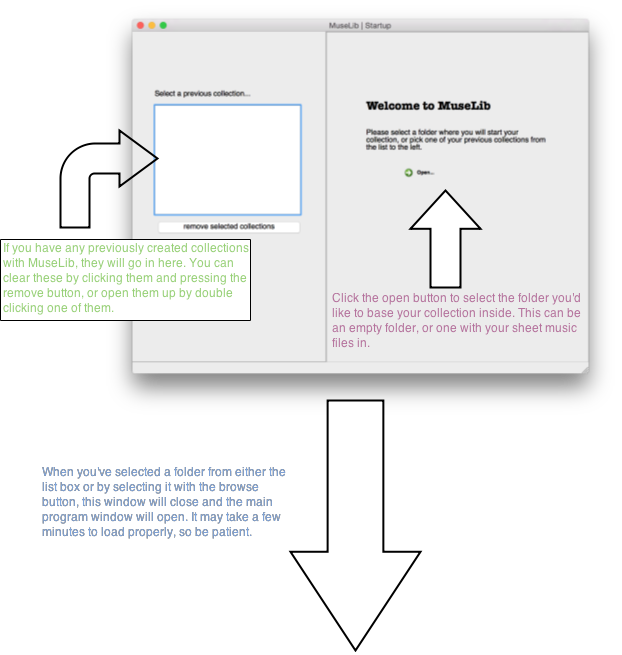
\includegraphics[width=400pt]{startup}
\caption{The window which will display on startup}
\label{fig:startup}	
\end{figure}

\subsection{Main view}
After the program has loaded, the main window shown in figure \ref{fig:main} will display. Panels to the left of this pane show a full listing of the files in your collection, which can be sorted by title, composer or lyricist, followed by a pane which displays any playlists you have created, followed by a third pane displaying playlists the system has generated for you. The auto generated playlists will automatically update with new pieces when you press the "refresh collection" option, located in the file menu.
\begin{figure}[H]
\centering
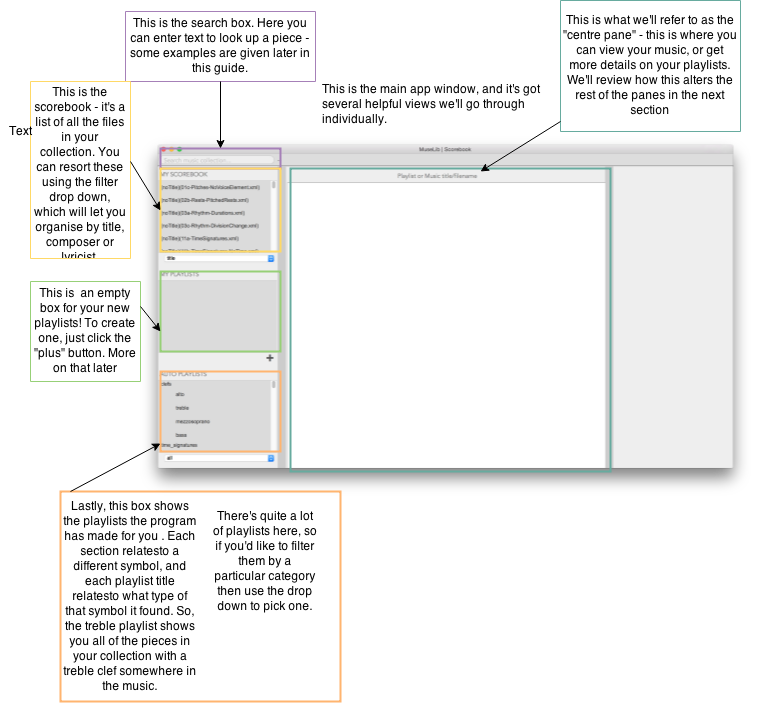
\includegraphics[width=500pt]{main_screenshot}
\caption{The window which will display on startup}
\label{fig:main}	
\end{figure}
\subsubsection{The User Created Playlist Widget}
The second widget from the top on the left is called the user created playlist widget. This will display all of the playlists you have created, as shown in figure \ref{fig:createdplaylists}. 
\begin{figure}[H]
\centering
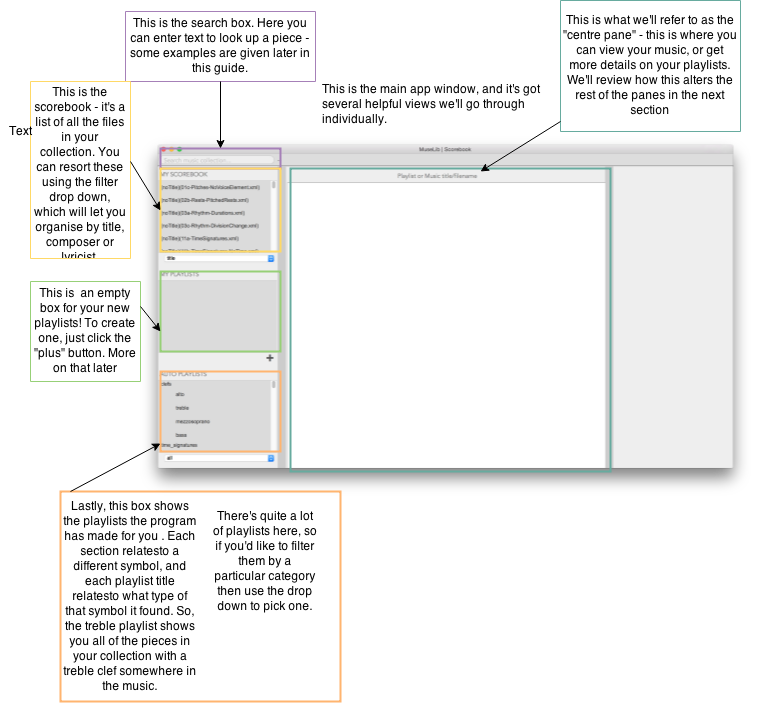
\includegraphics[width=500pt]{main_screenshot}
\caption{Window with playlists created by a user listed in second widget}
\label{fig:createdplaylists}	
\end{figure}

To add a new playlist to this list, press the add button, and a new popup will display as shown in figure \ref{fig:newplaylist}. Enter a title for this playlist, and search for pieces. The search functionality of this window is the same as the main window, as explained in section 2.3, so enter any information about the piece such as time signature, key etc in the same way you would in the main search box. These will be listed in the listbox below the text entry box, and can be reordered by dragging. Pieces can be removed from this list by selecting the item and pressing delete.
\begin{figure}[H]
\centering
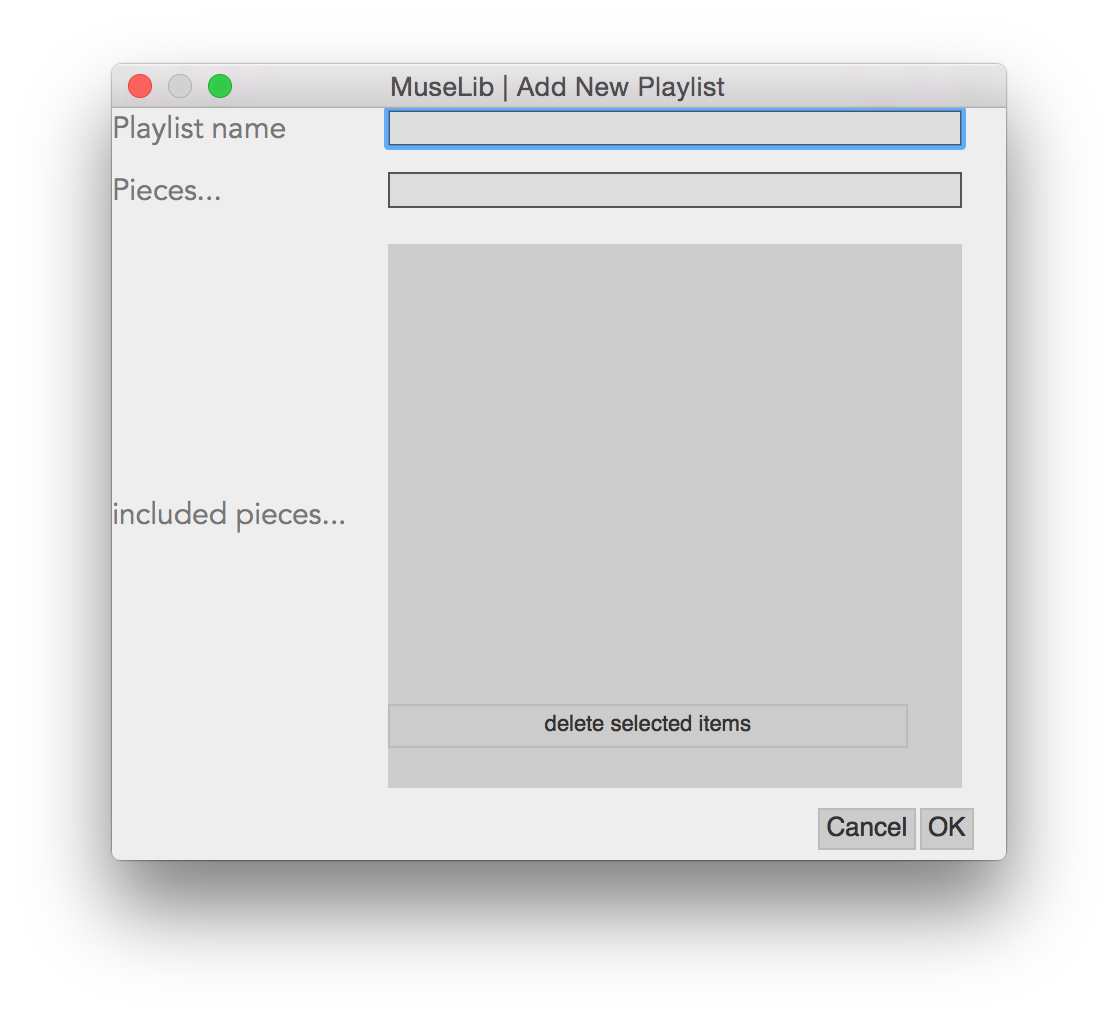
\includegraphics[width=\textwidth]{playlistpop}
\caption{Popup window for creating new playlists}
\label{fig:newplaylist}	
\end{figure}
Finally, press OK and the playlist will display in the widget to the left.

\subsection{Searching}
The search box at the top of the application allows you to browse your collection by entering information about the piece, as shown in figure \ref{fig:search}.
\begin{figure}[H]
\centering
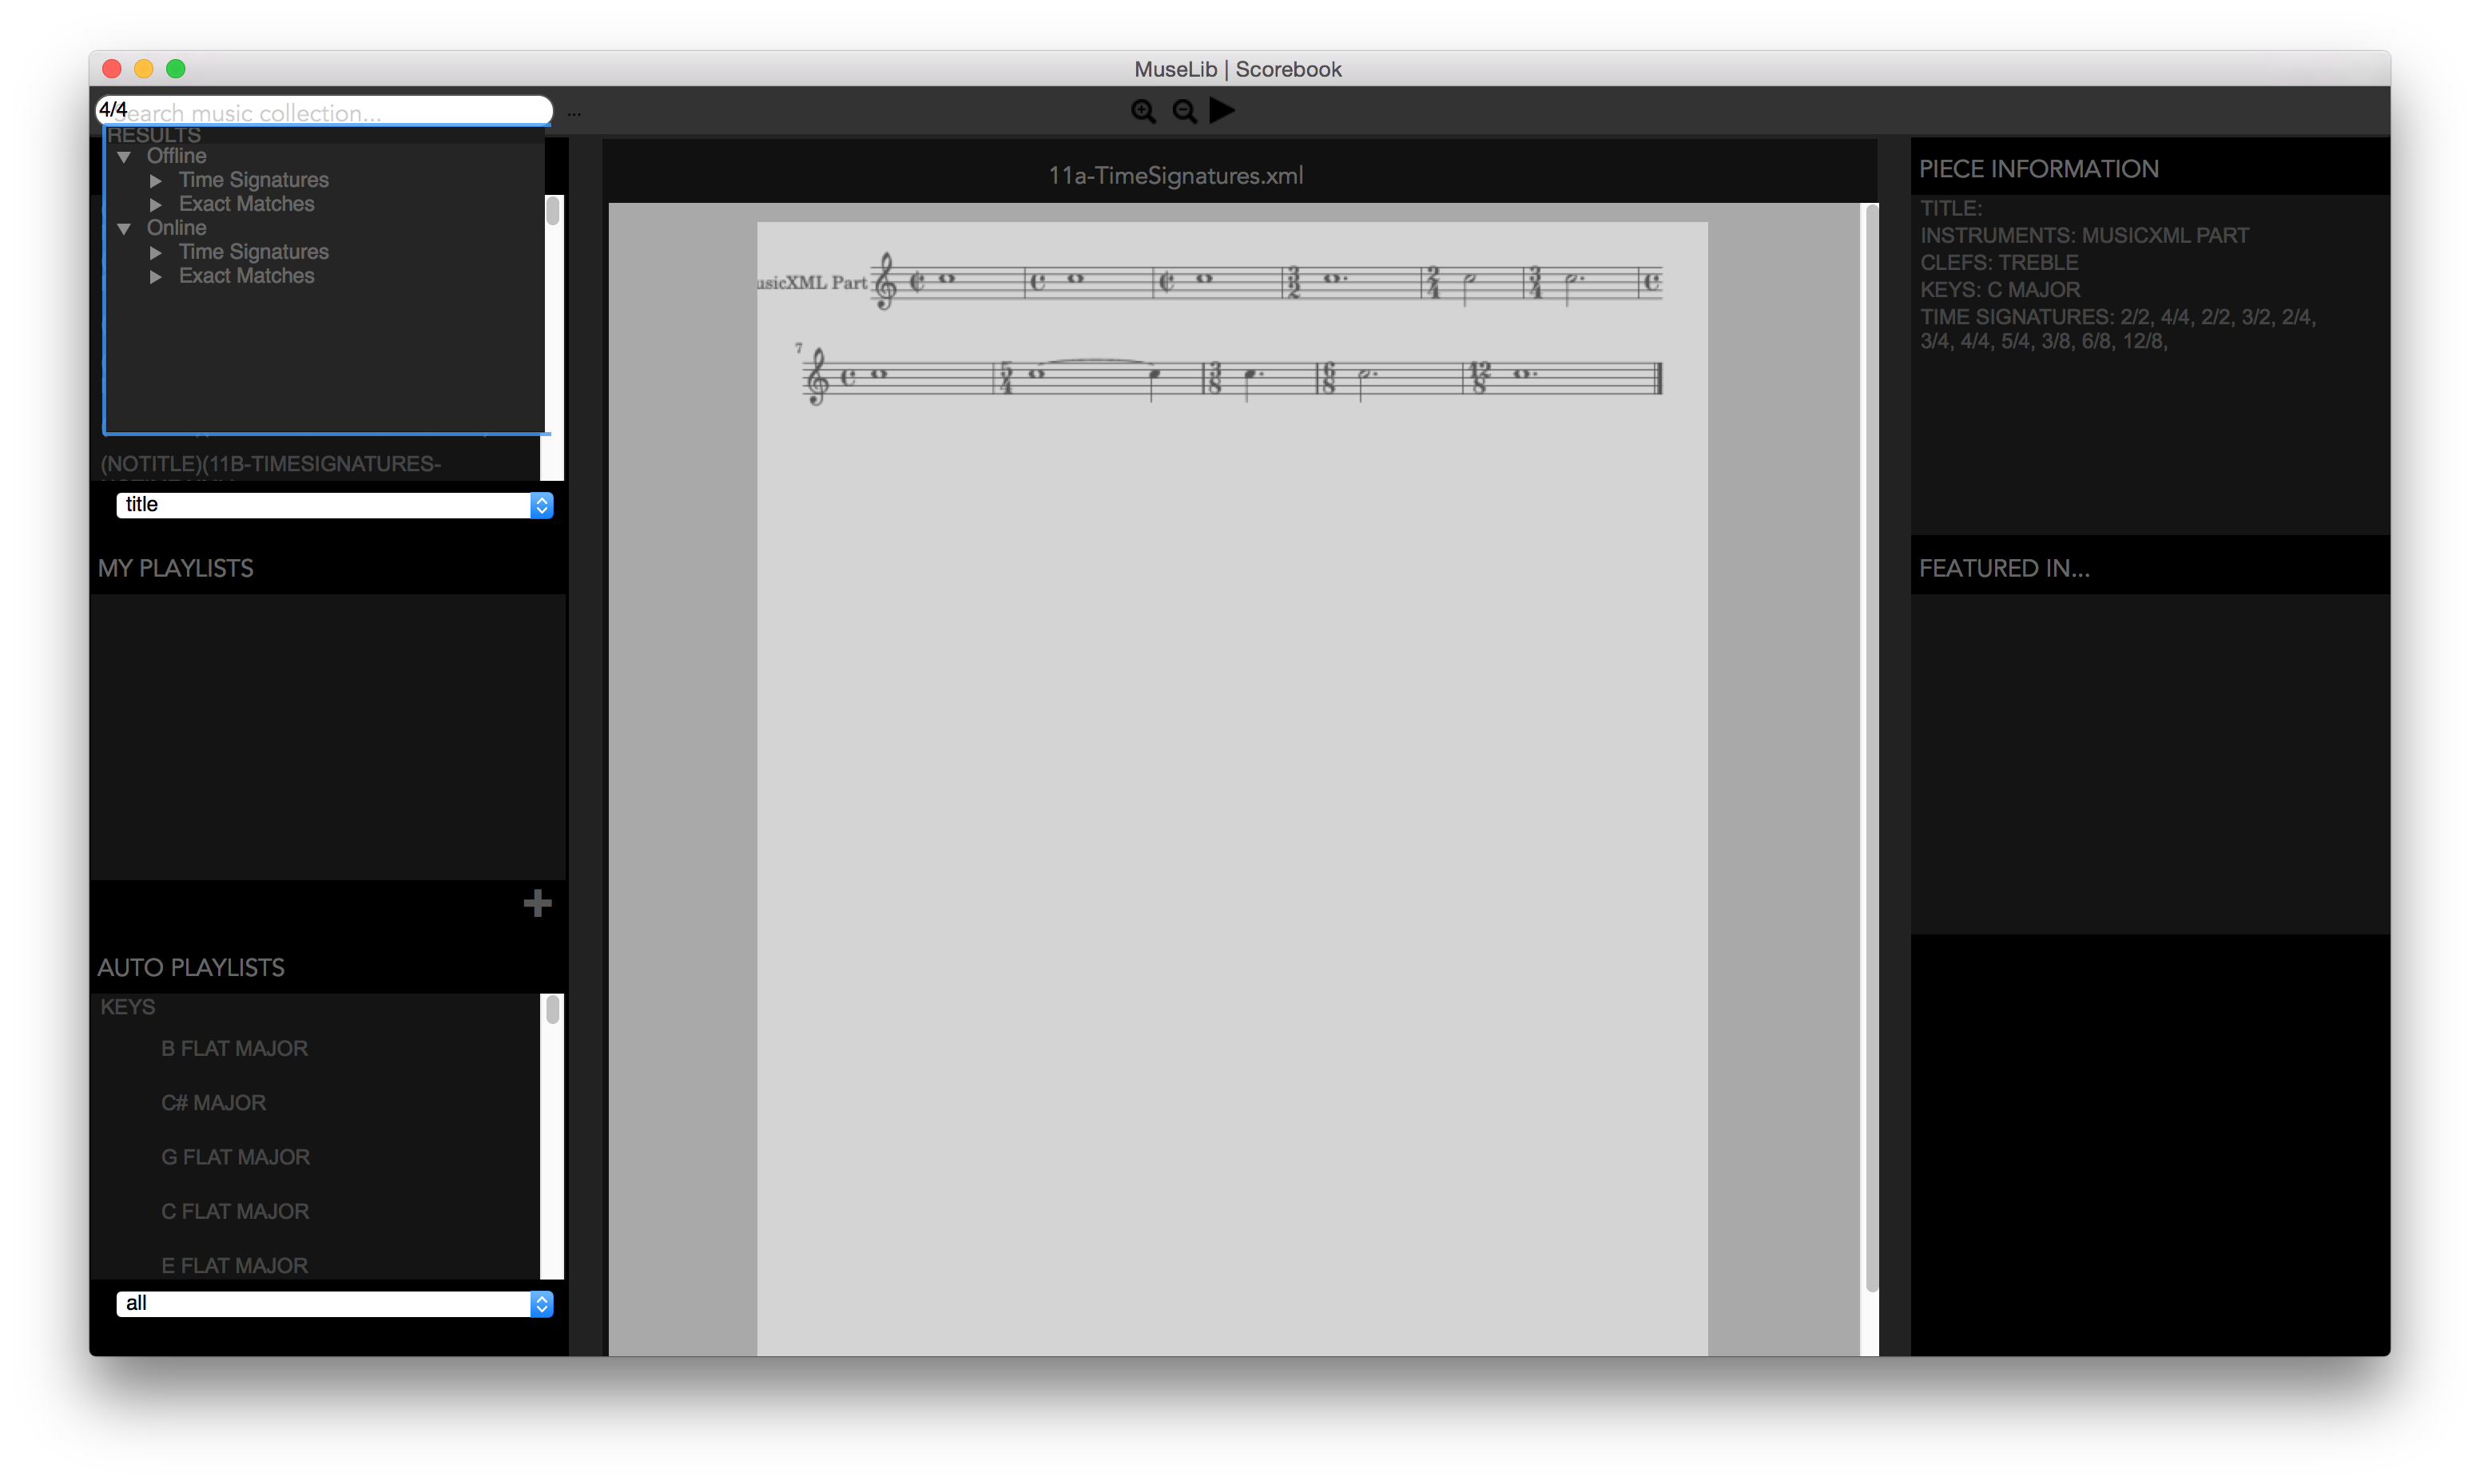
\includegraphics[width=500pt]{main_results}
\caption{Main window with search input results displaying}
\label{fig:search}	
\end{figure}

\subsubsection{Simple Searches}
In some instances, such as the query above, you may enter text into the box without needing to tell the system what you are looking for. Table \ref{table:commands} shows some of the commands you can use, separated by spaces.

\begin{table}[H]
\begin{tabu} to 1.05\textwidth {| X[l] | X[c] |} \hline
{Command} & {Result} \\ \hline
$<$letter$><$space$>$ followed by Major or Minor & System will look for pieces in this key (ignoring transposing instruments) \\ \hline
$<$number$>$/$<$number$>$ & System will search for a time signature \\ \hline
$<$rhythmicname$>$=$<$value$>$ & System will search for a tempo, where rhythmic name means quarter/crotchet, half/minim etc. \\ \hline
Text abc def & System will search individually for any pieces where the file name, title, composer, instrument names or lyricist match any of the individual words \\ \hline
"My name is fred" & System will search for the exact quote in all of the above \\ \hline
\end{tabu}
\caption{A table describing the command options for simple searches}
\label{table:commands}
\end{table}

\subsubsection{Complex Searches}
The structure laid out in section 2.3.1 manages to predict the majority of searches you might want to enter. However, some queries require more complexity, and as such "labels" are provided in order to achieve this. These are given in table \ref{table:commands_complex}.
\begin{table}[H]
\begin{tabu} to 1.05\textwidth {| X[l] | X[l] |} \hline
{\textbf{Command}} & {\textbf{Result}} \\ \hline
key:"C major" & System will look for pieces in this key \\ \hline
clef:treble & System will look for pieces with this clef in any part \\ \hline
meter:4/4 & System will search for a time signature \\ \hline
instrument:clarinet with:key:"C major" & System will search for pieces containing the instrument "clarinet" which is in the key of C major at some point in the piece \\ \hline
instrument:clarinet with:clef:bass & System will search for pieces containing the clarinet where the clarinet has a bass clef somewhere in the piece \\ \hline
instrument:clarinet with:clef:bass;key:"C major" & System will search for pieces containing the clarinet where the clarinet has a bass clef somewhere in the piece and is in C major somewhere in the piece \\ \hline
transposition:clarinet with:clef:bass;key:"C major" & System will search for pieces containing the clarinet, or if there is no clarinet, any instrument which has the same transposition \\ \hline
\end{tabu}
\caption{A table describing the command options for complex searches}
\label{table:commands_complex}
\end{table}

\subsubsection{Downloading new files}
When you search for files, the system will also provide you with suggestions which are located in online collections. You may choose to add these files to your collection simply by double clicking. This will open up a popup box as shown in figure \ref{fig:license}, which shows the license terms for that particular piece. When you click OK, the system will download and display the file.
\begin{figure}[H]
\centering
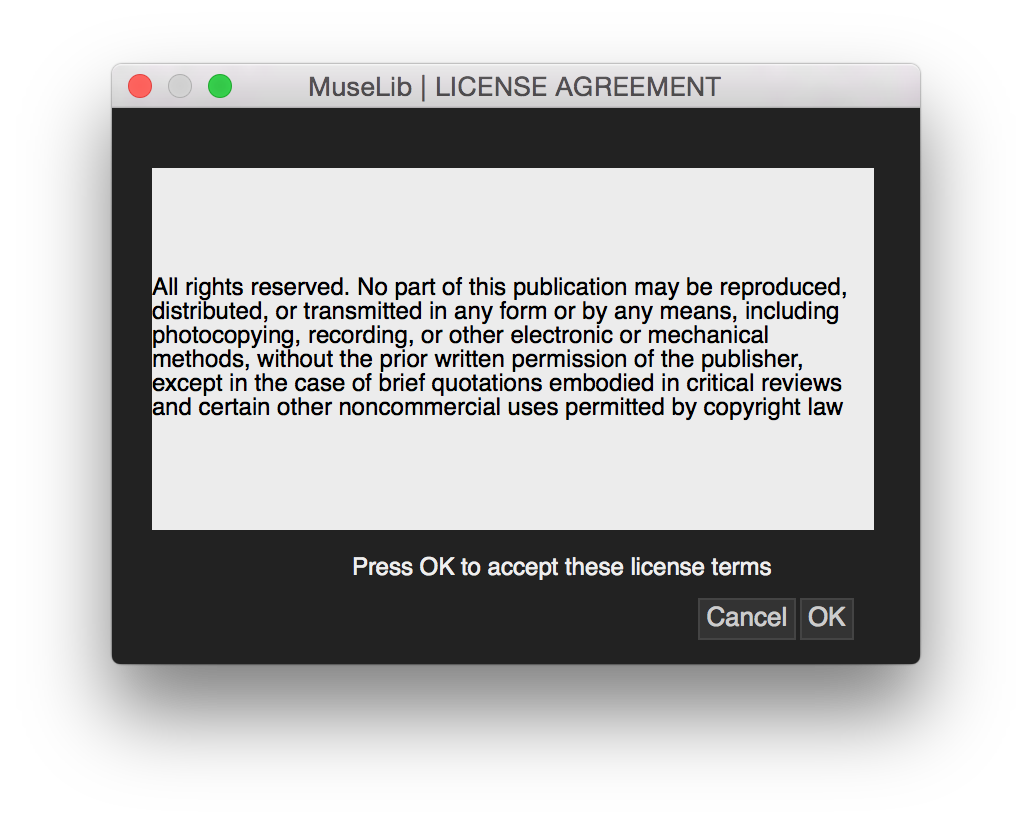
\includegraphics[width=400pt]{licensepop}
\caption{The popup which displays when a piece downloads}
\label{fig:license}	
\end{figure}

\subsection{Piece view}
When you view a piece, it will display in the middle portion and update the panes to the right according to data found, as shown in figure \ref{fig:piece}. The first pane to the right is for information about this piece. This displays all the information the system knows about the given piece.
The second pane displays any playlists you have created which feature this piece.
The third pane is a minimised version of the playlist browser. This will only display if you loaded this piece from the playlist view, as shown in figure \ref{fig:playlist}

\begin{figure}[H]
\centering
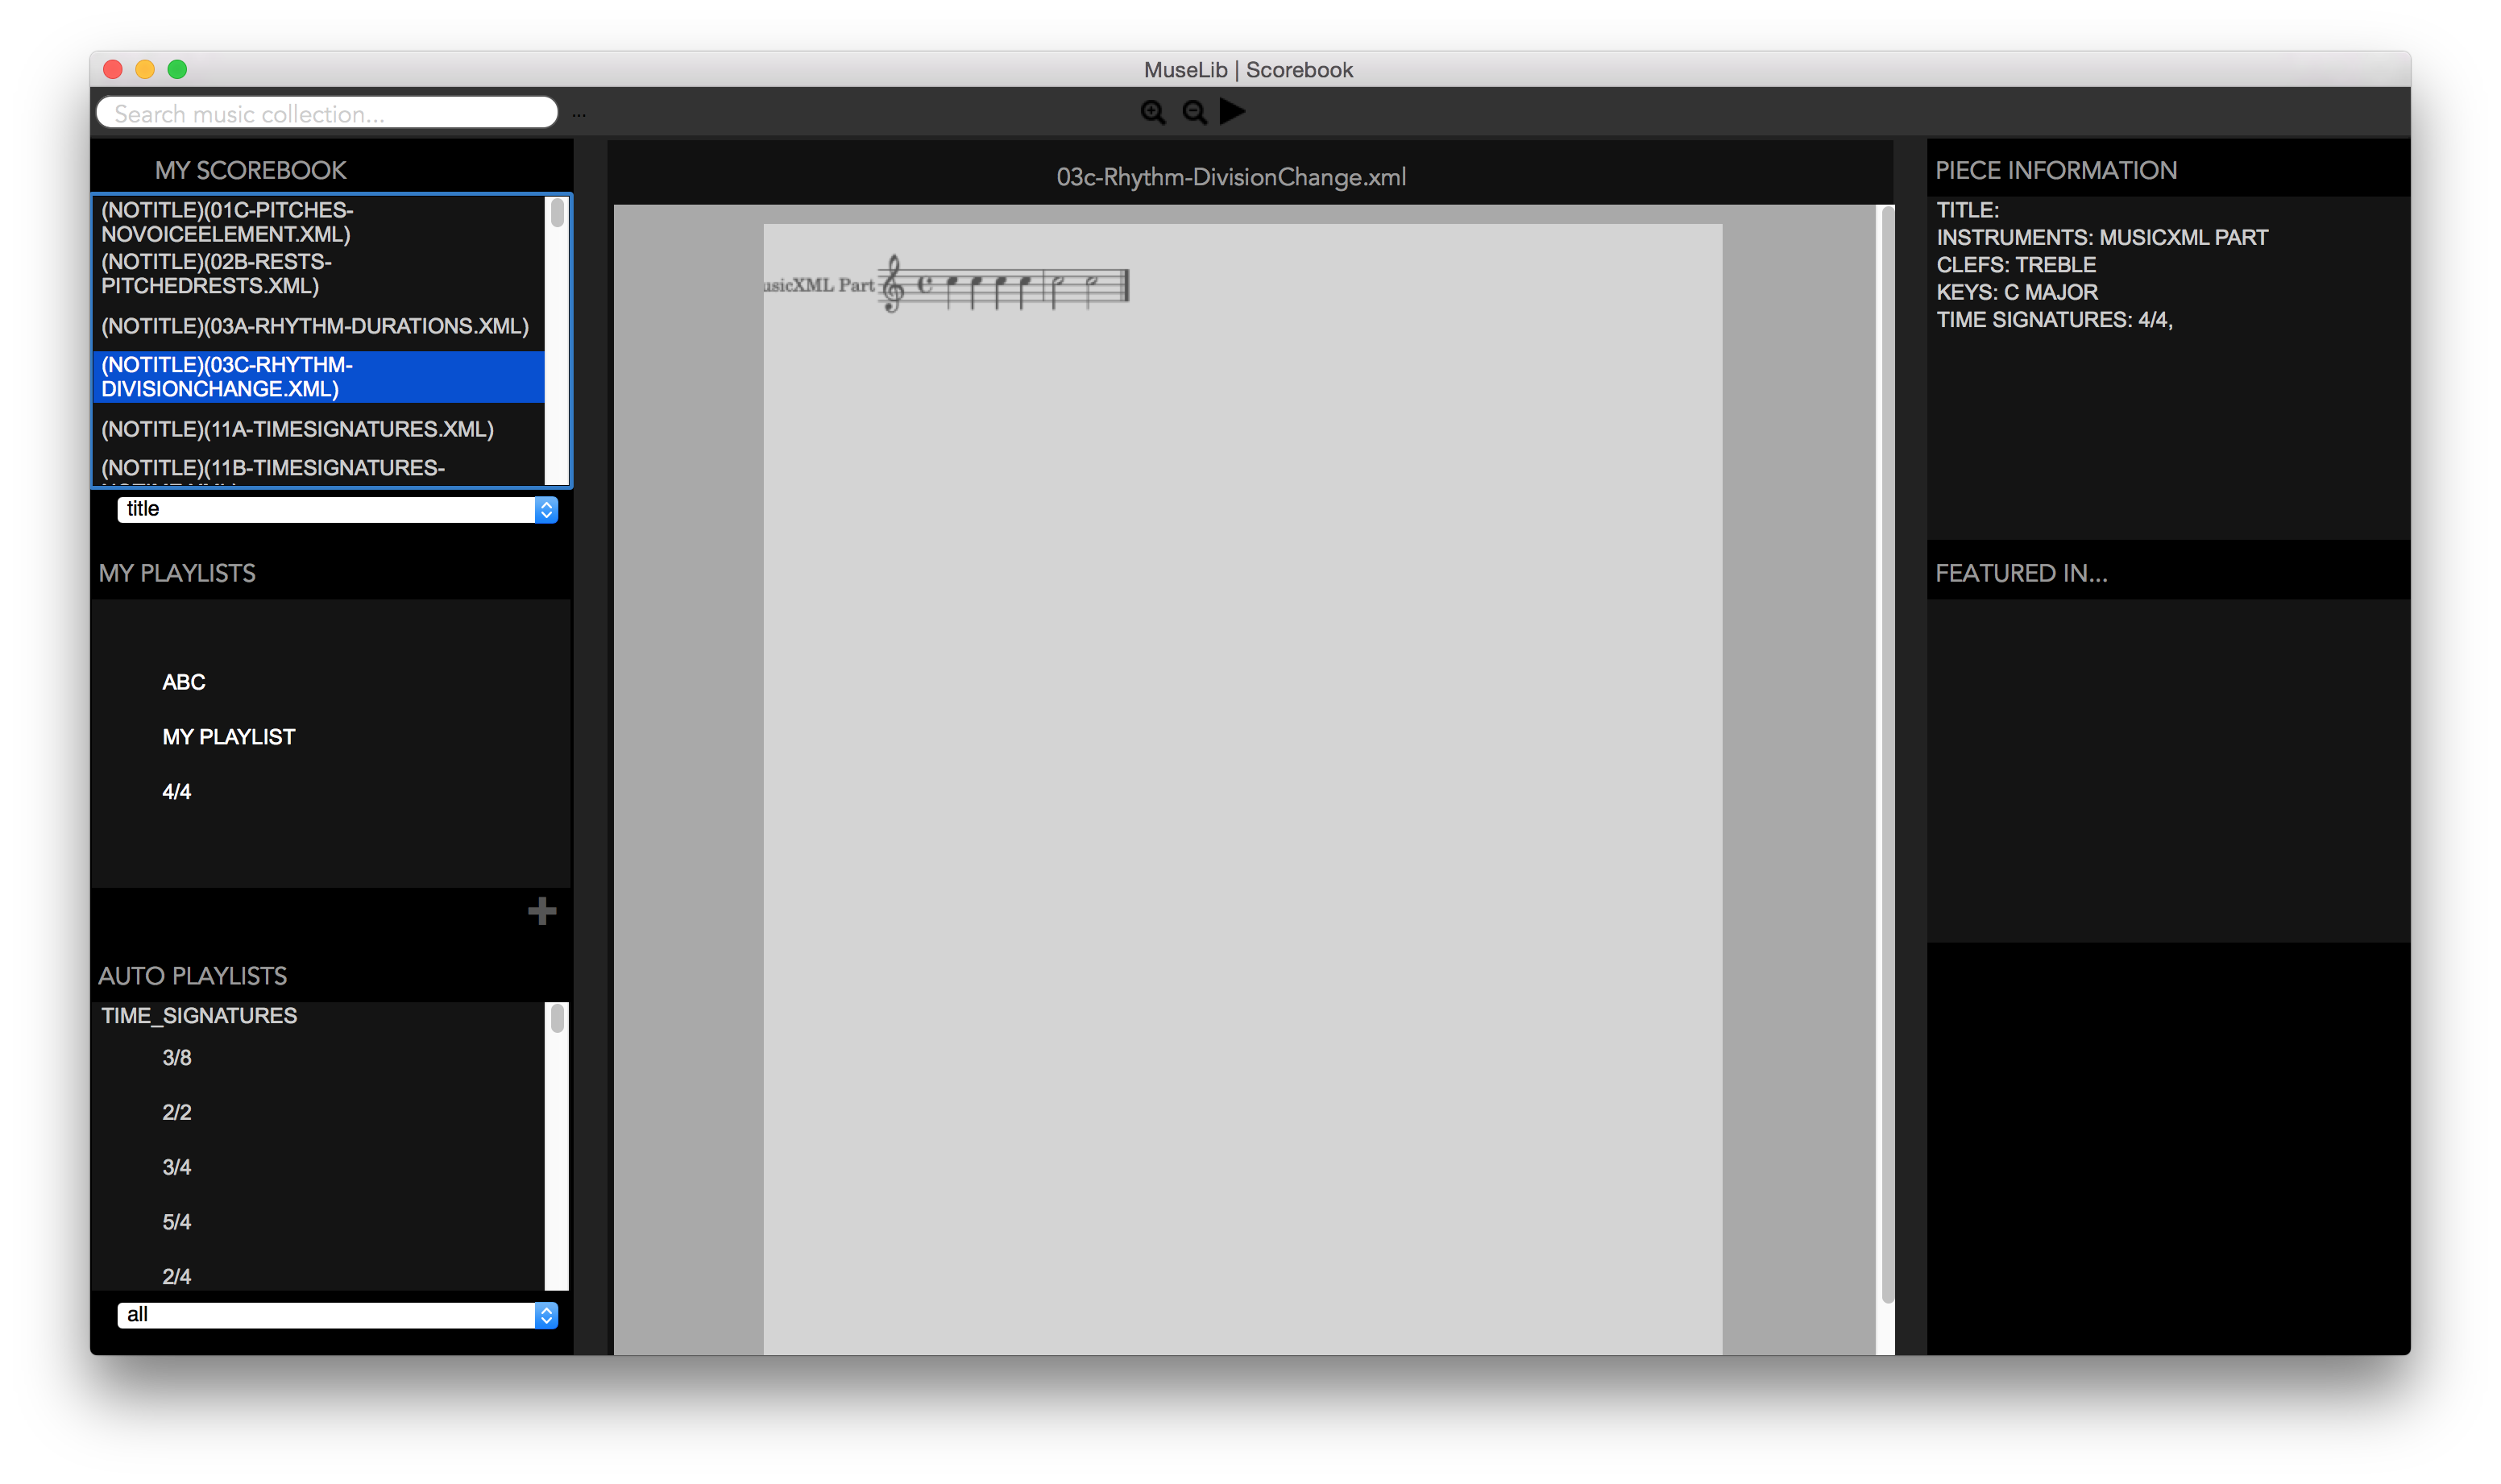
\includegraphics[width=500]{main_piece}
\caption{The main view showing a loaded piece}
\label{fig:piece}	
\end{figure}

There are also two buttons above the piece of music, the first of which allows you to zoom in, and the second zoom out. The third button is a feature which has yet to be put in.
\subsection{Playlist View}
When you select a playlist from either the user created widget or the auto generated playlists widget, the main window will update as shown in figure \ref{fig:playlist}. This displays a full list of pieces in the playlist together with all of the associated data.
\begin{figure}[H]
\centering
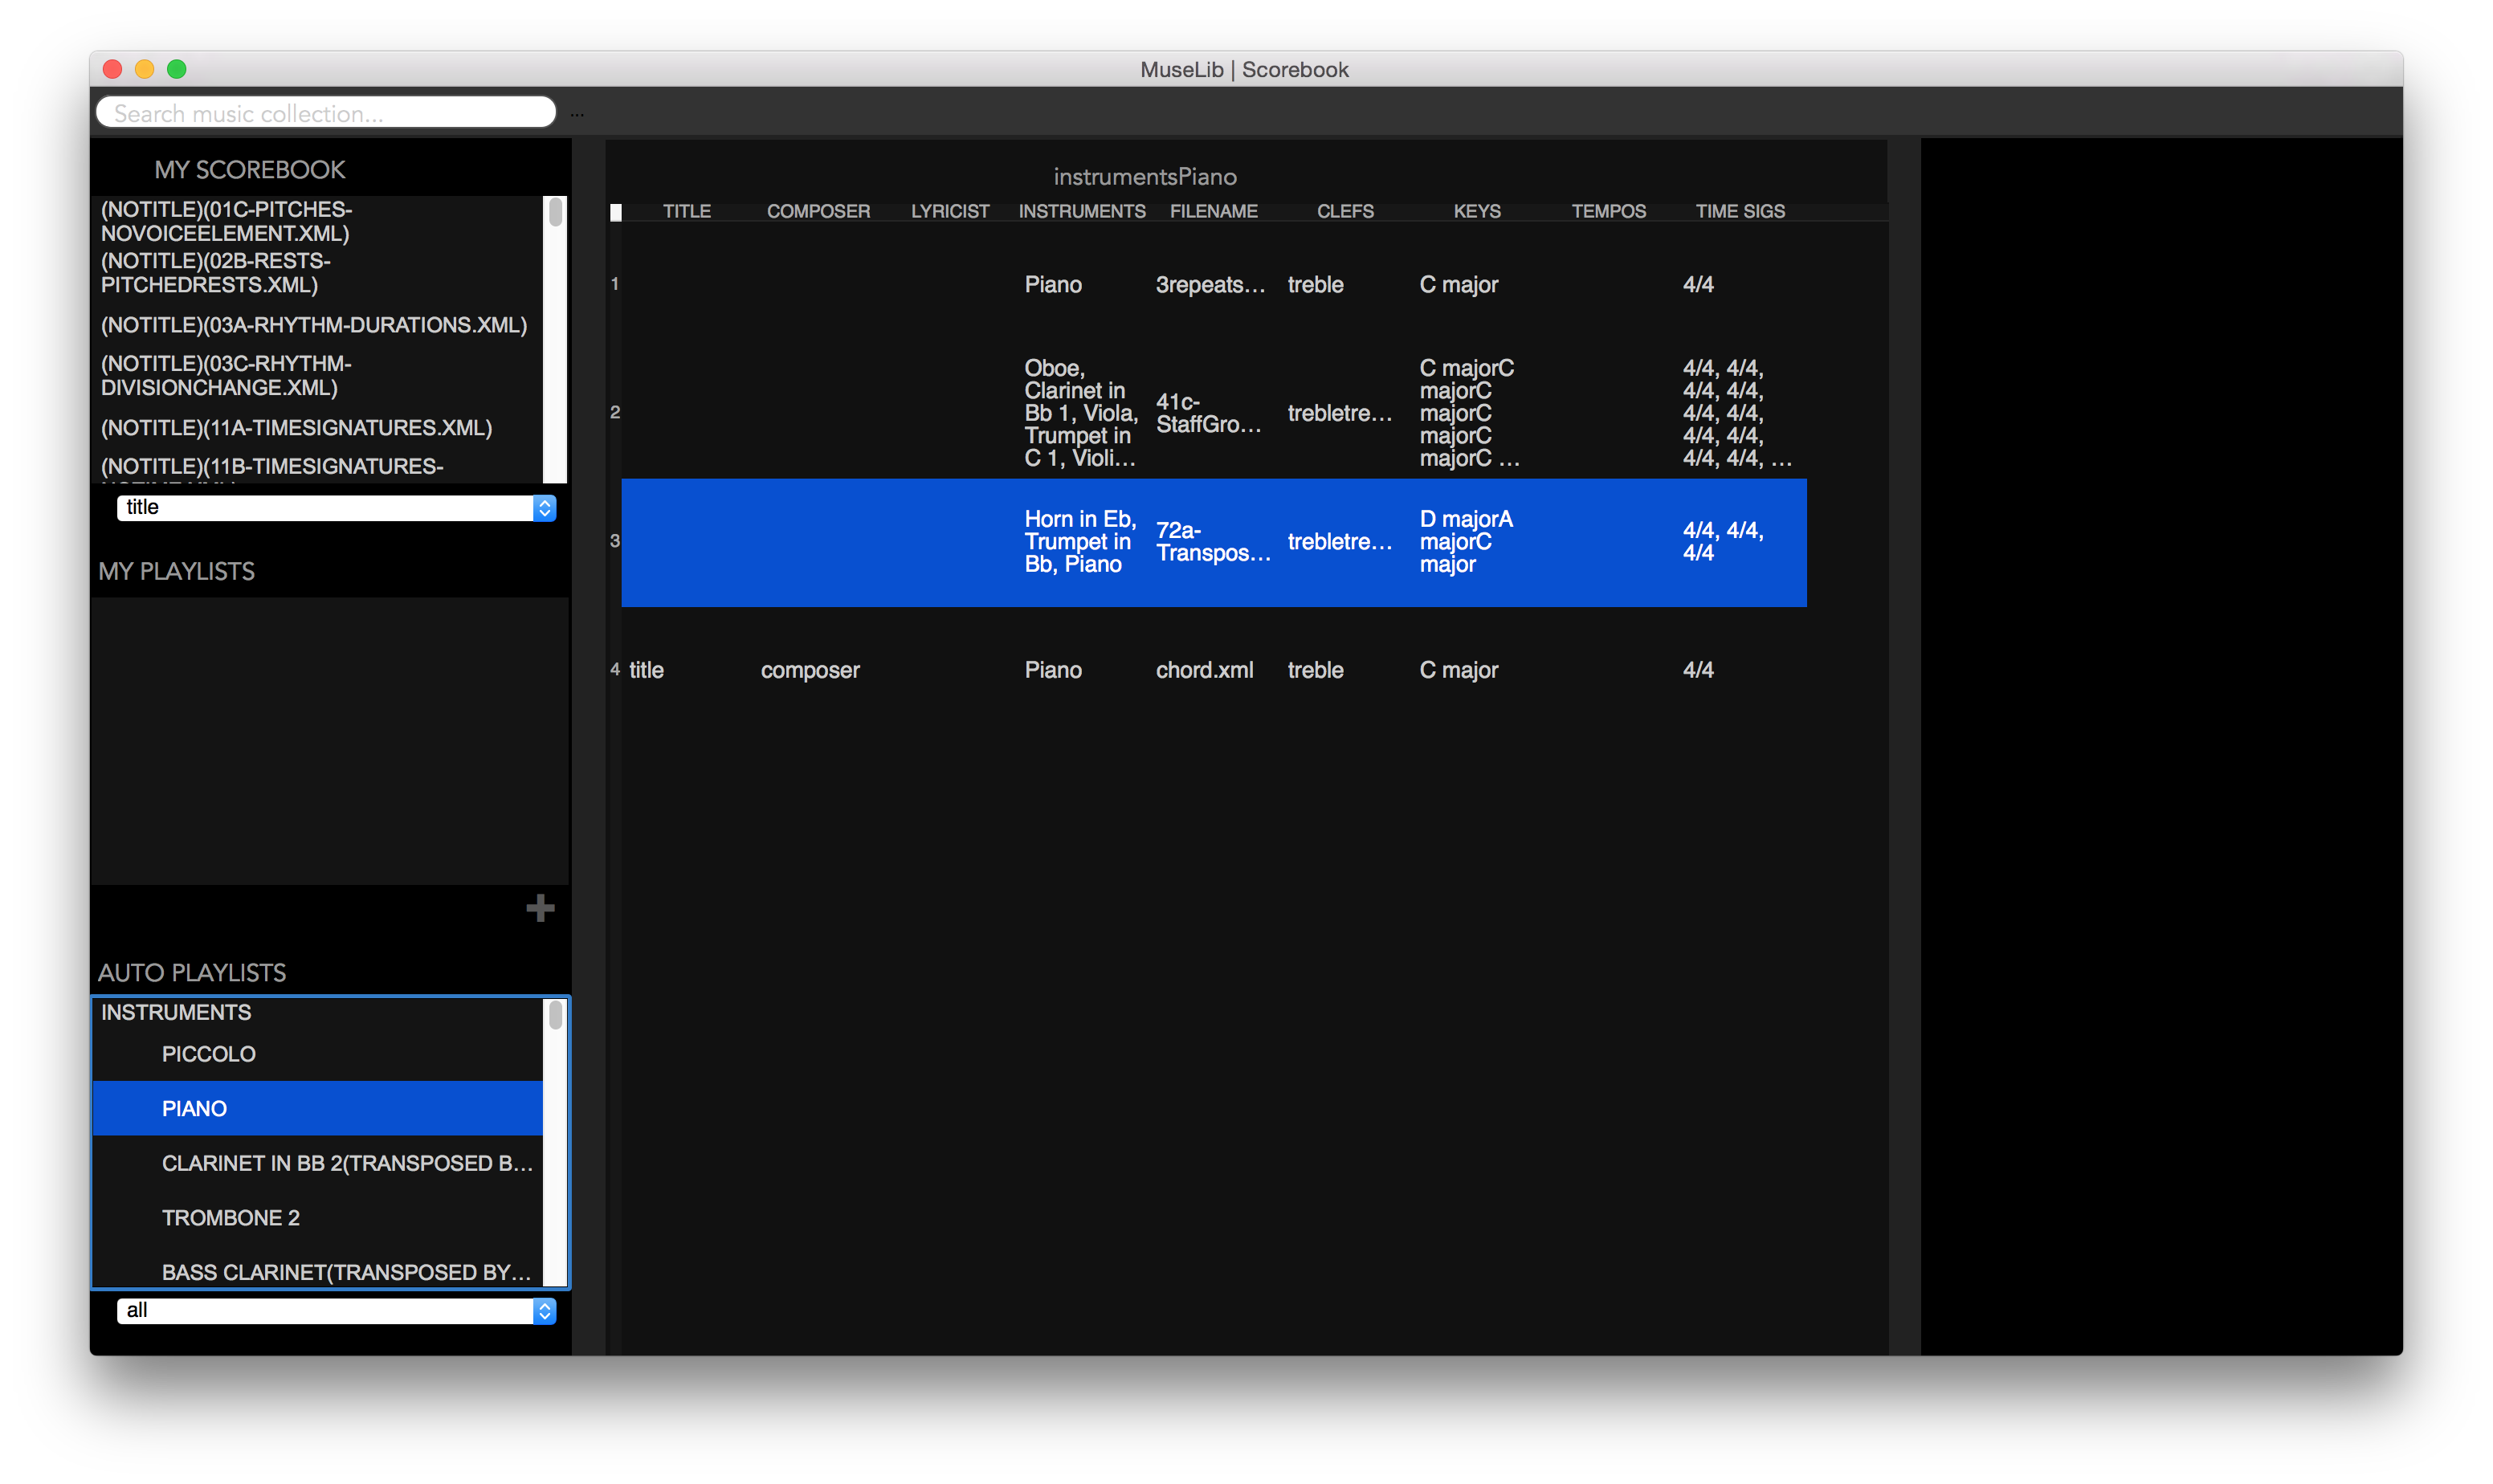
\includegraphics[width=500pt]{main_playlist}
\caption{The playlist view}
\label{fig:piece}	
\end{figure}

\subsubsection{Viewing a piece from the playlist view}
When you double click any of the pieces in a given playlist, the view will update as shown in figure \ref{fig:playlistbrowser}. A third widget has been displayed on the right, showing a full listing of the playlist. The widget has also highlighted the current piece you have selected.
\begin{figure}[H]
\centering
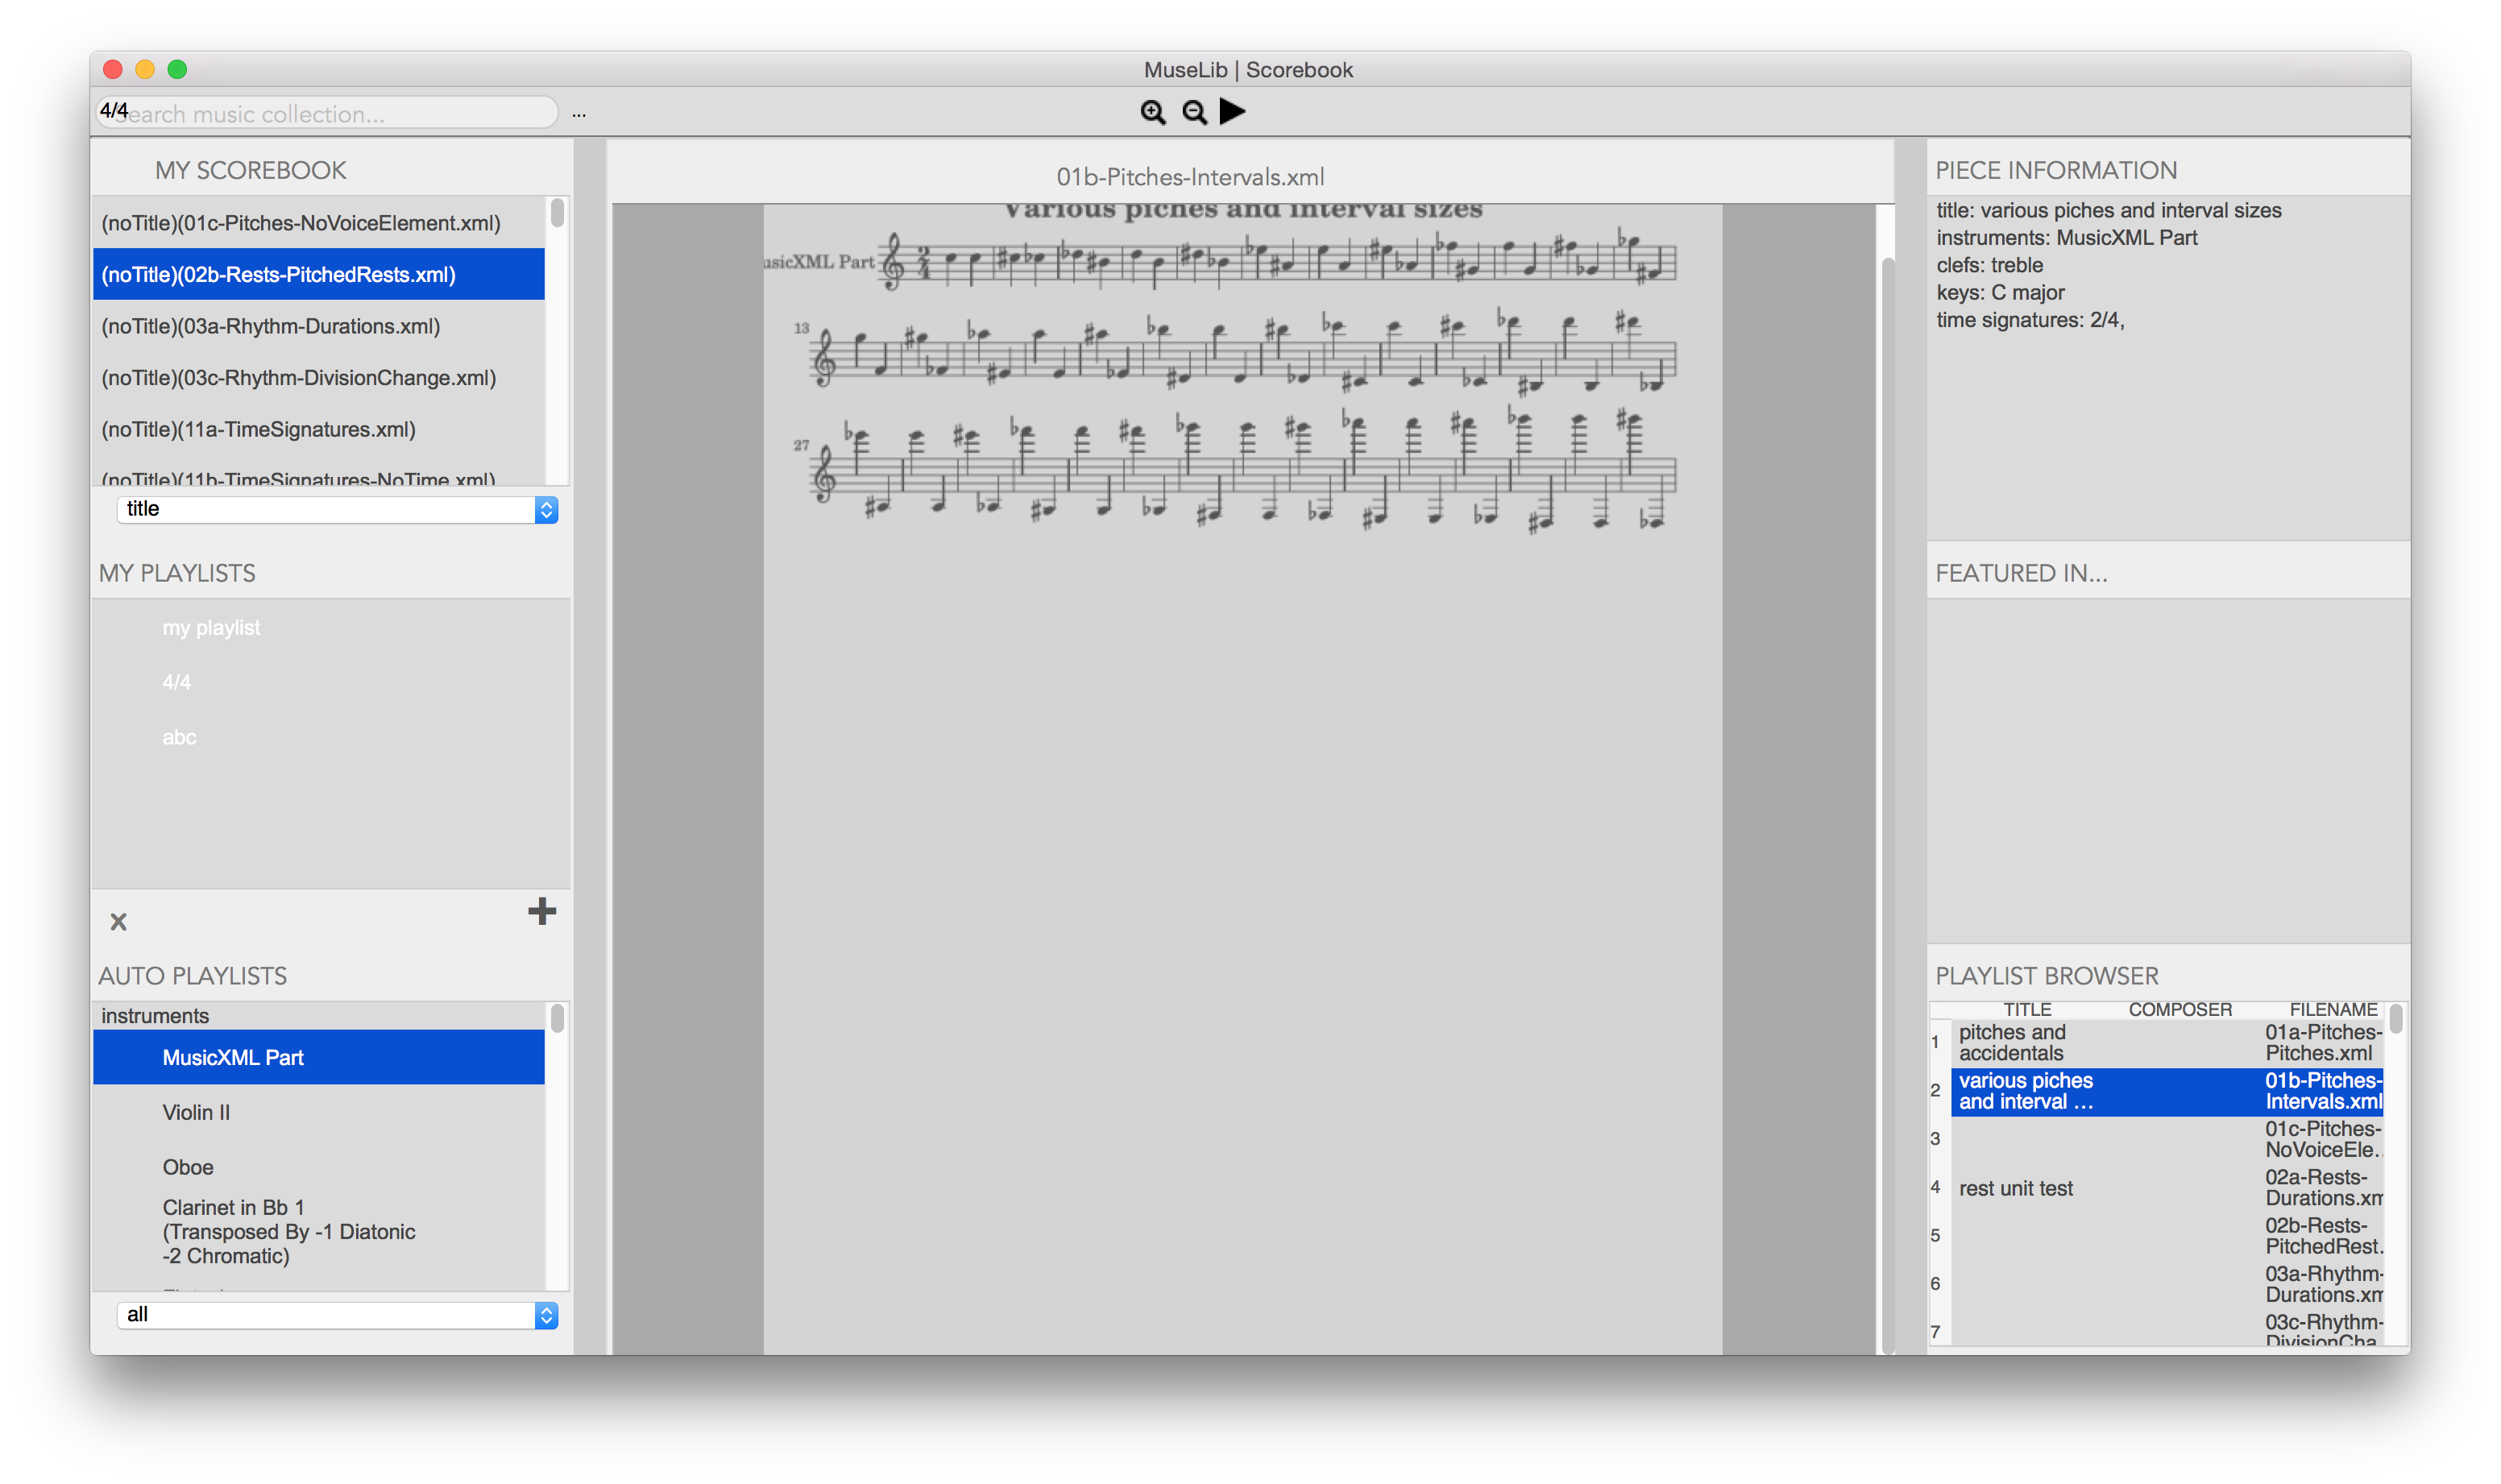
\includegraphics[width=500pt]{playlistbrowser}
\caption{The window which will display on startup}
\label{fig:playlistbrowser}	
\end{figure}

\subsection{Popups and Error Windows}
\subsubsection{The Import Popup}
If you wish to add a new file from inside the application which does not reside in the main collection folder, you may import it using the import window. To open it go to File->Import from the main window. The popup in figure \ref{fig:import} will display.
\begin{figure}[H]
\centering
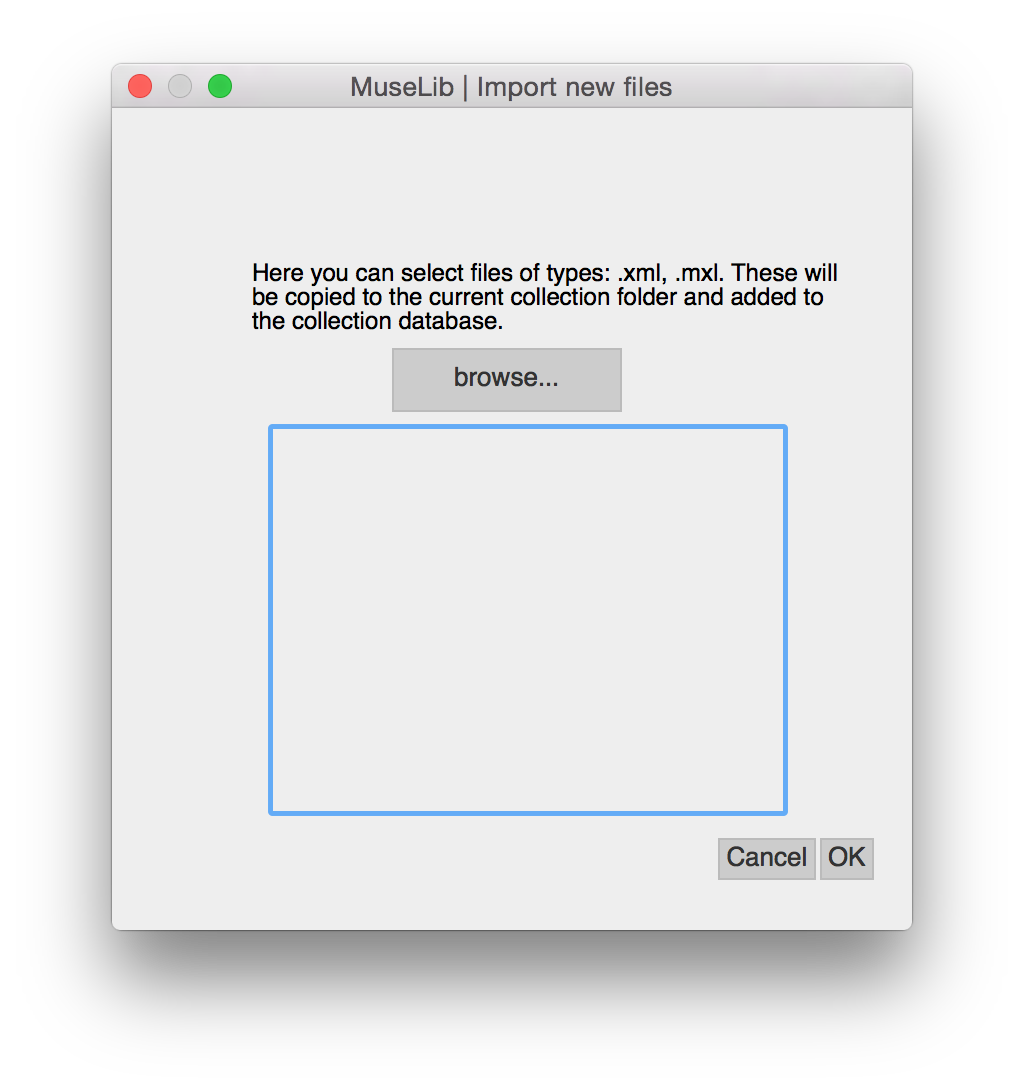
\includegraphics[width=500pt]{importpop}
\caption{The import popup window}
\label{fig:import}	
\end{figure}
Click browse to find the file. This window will allow you to select multiple files by browsing for one, selecting it and then browsing again. The list of files to copy will display in the listbox below the button.


\subsubsection{Error Popup}
Occasionally, files produce problems the system cannot handle - this includes drum tab and guitar tab. At other times there will be problems in the process the application could not process for different reasons, such as downloading files without internet connection. When these occur, the popup in figure \ref{fig:error} will display. If you find any odd errors, please report these to a developer.
\begin{figure}[H]
\centering
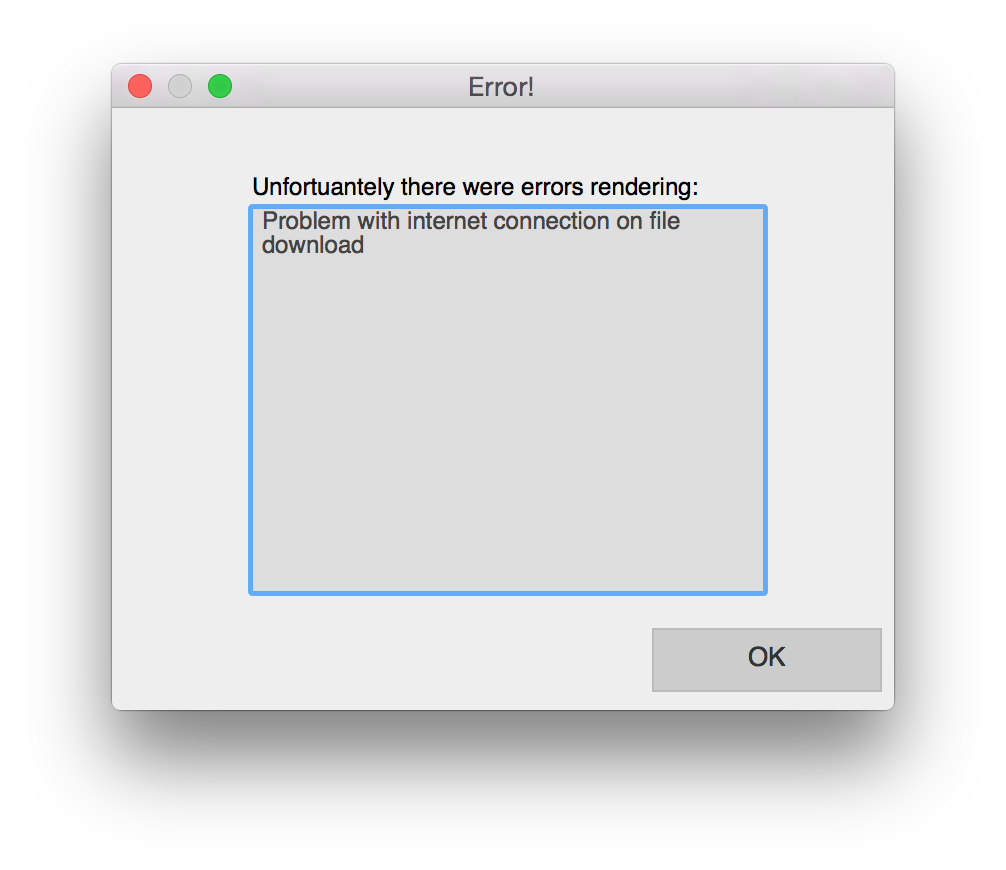
\includegraphics[width=500pt]{errorpop}
\caption{The window which will display on startup}
\label{fig:error}	
\end{figure}

\subsection{Customising your display}
\subsubsection{Themes}
The system comes with three different themes - the default which is light, dark and electric blue. These can be changed by clicking them in the theme menu as shown in figure \ref{fig:themes}. Their respective screenshots are shown in figures \ref{fig:theme1}, \ref{fig:theme2}, \ref{fig:theme3} and \ref{fig:theme4}.
\begin{figure}[H]
\centering
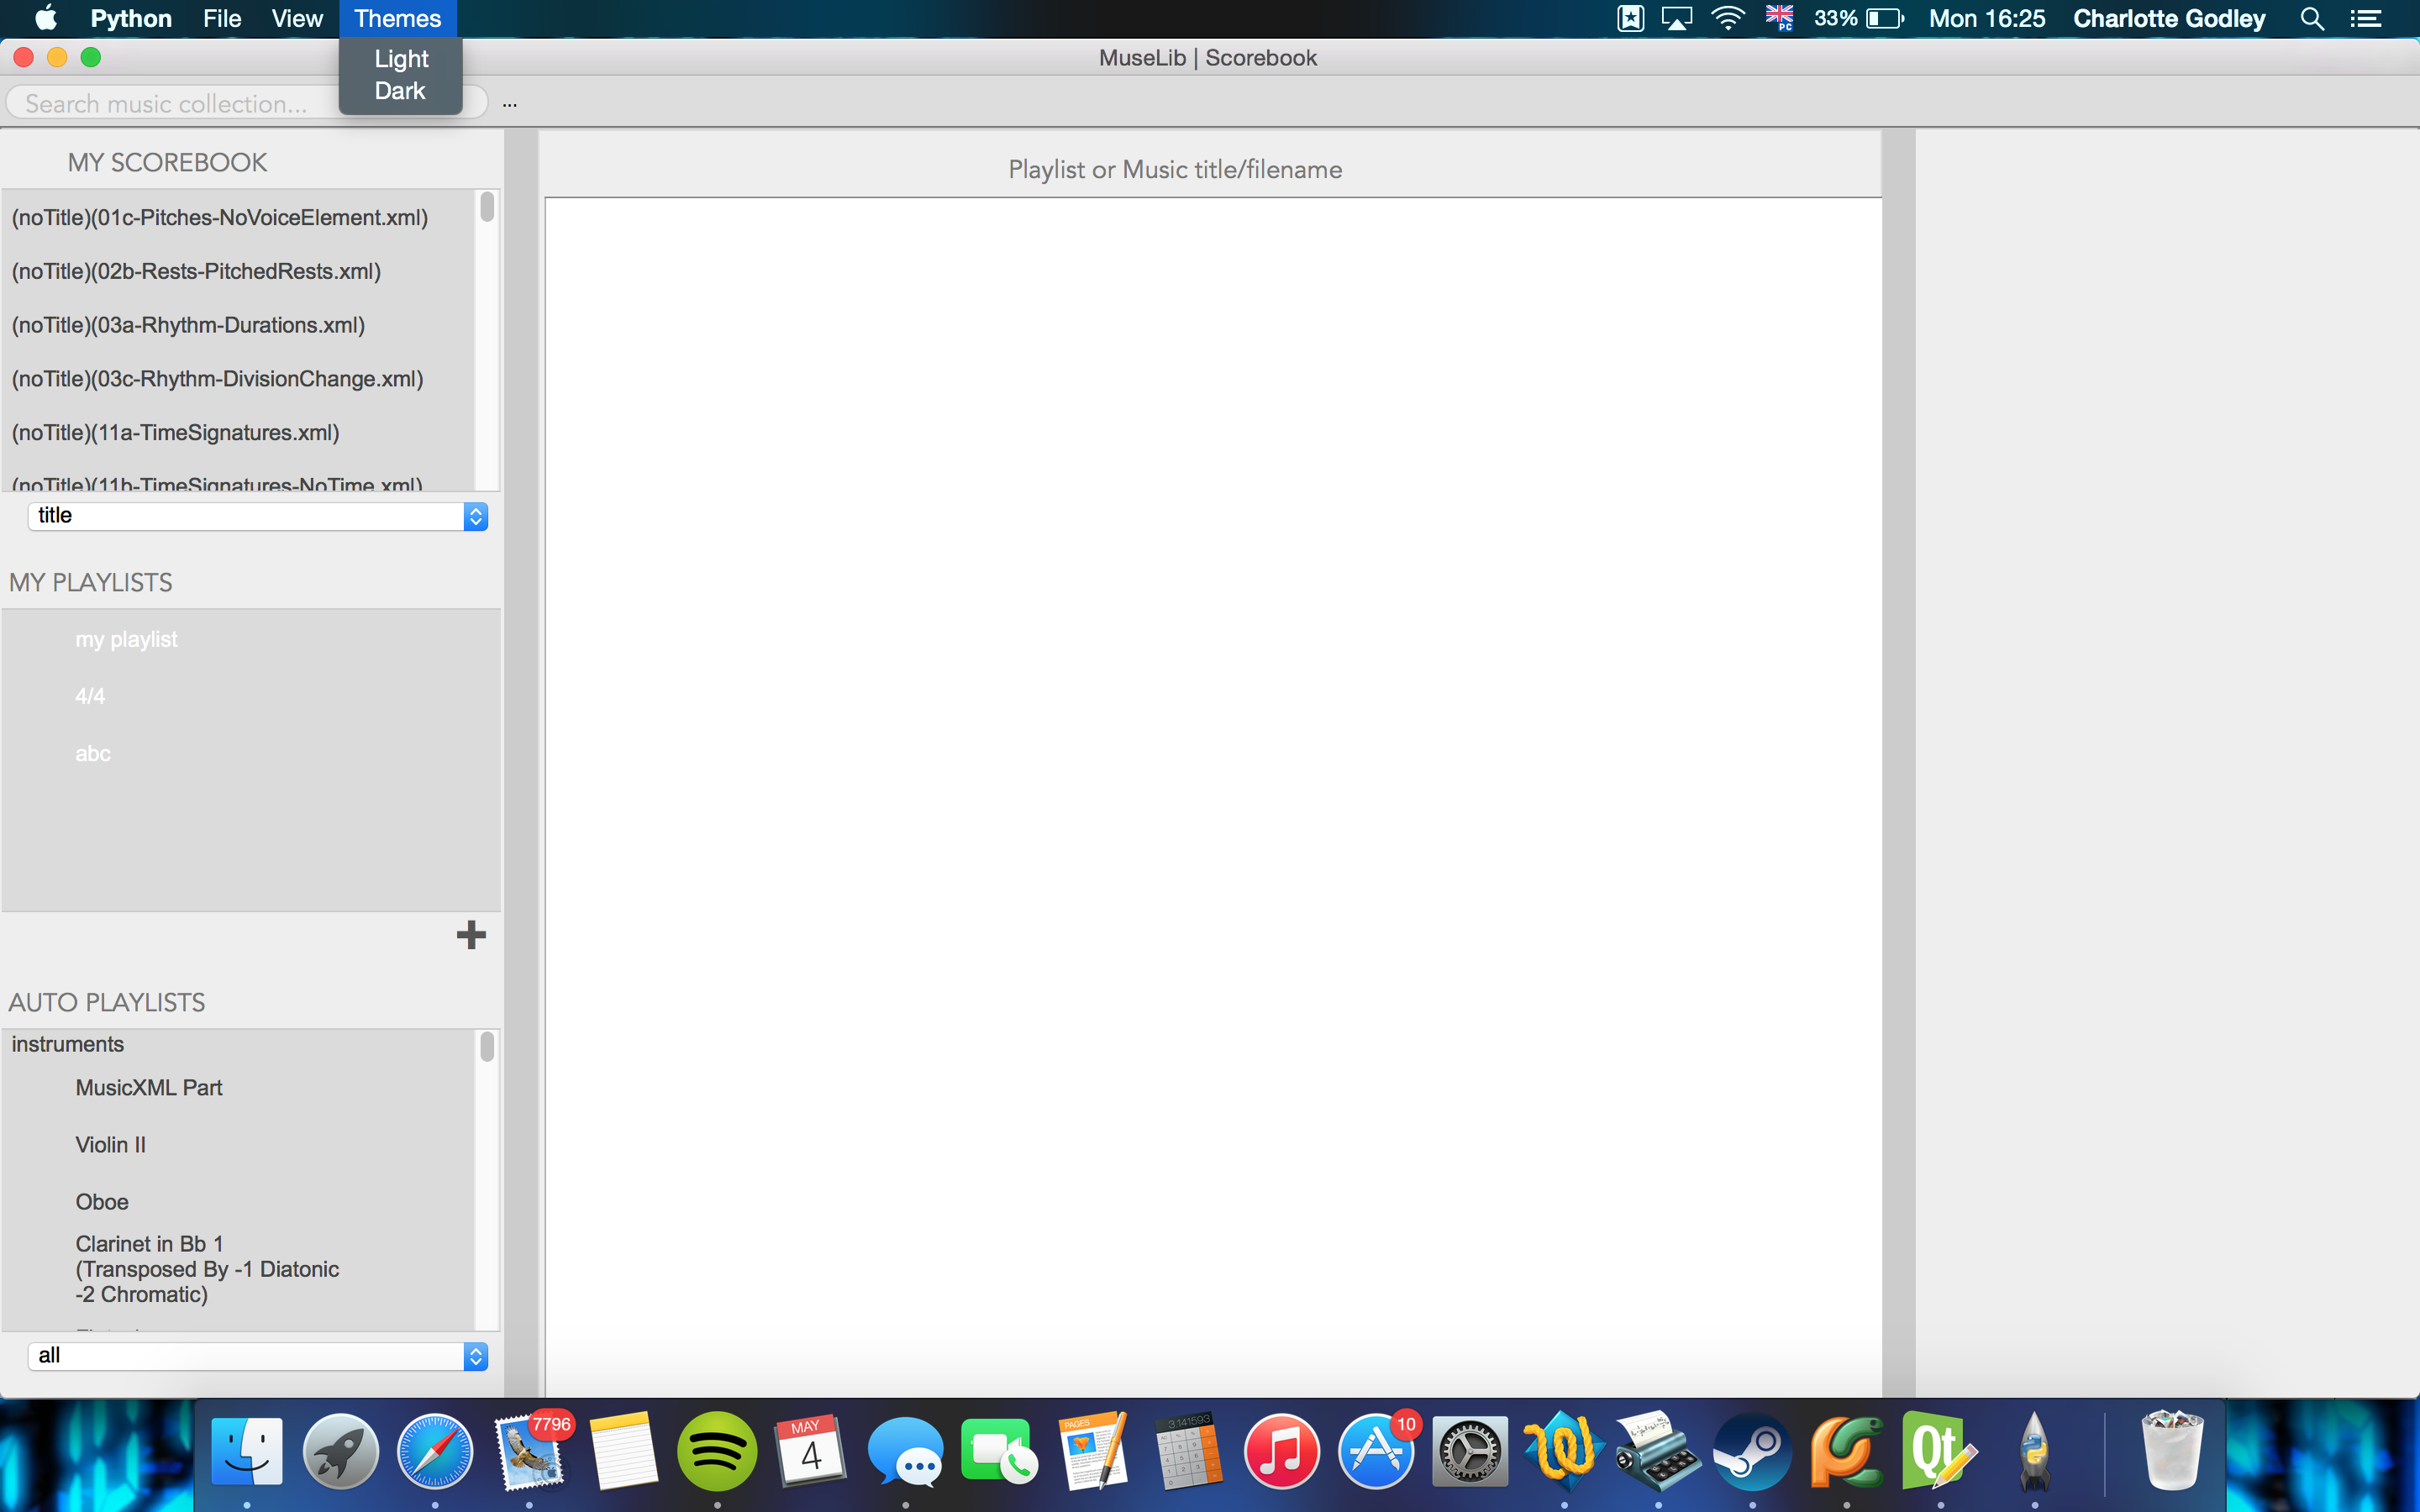
\includegraphics[width=500pt]{theme}
\caption{The themes menu}
\label{fig:themes}	
\end{figure}

\begin{figure}[H]
\centering
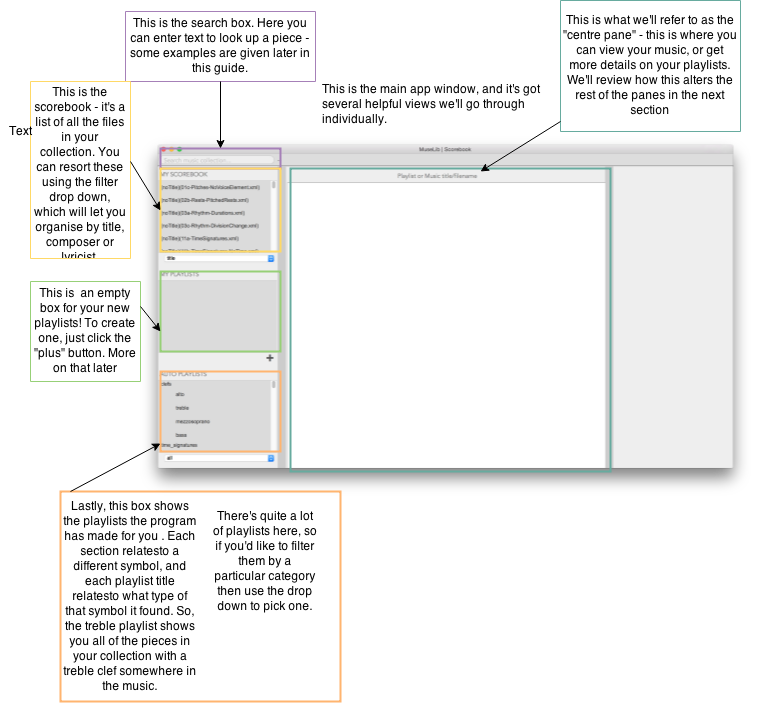
\includegraphics[width=400pt]{main_screenshot}
\caption{The light theme}
\label{fig:theme1}	
\end{figure}

\begin{figure}[H]
\centering
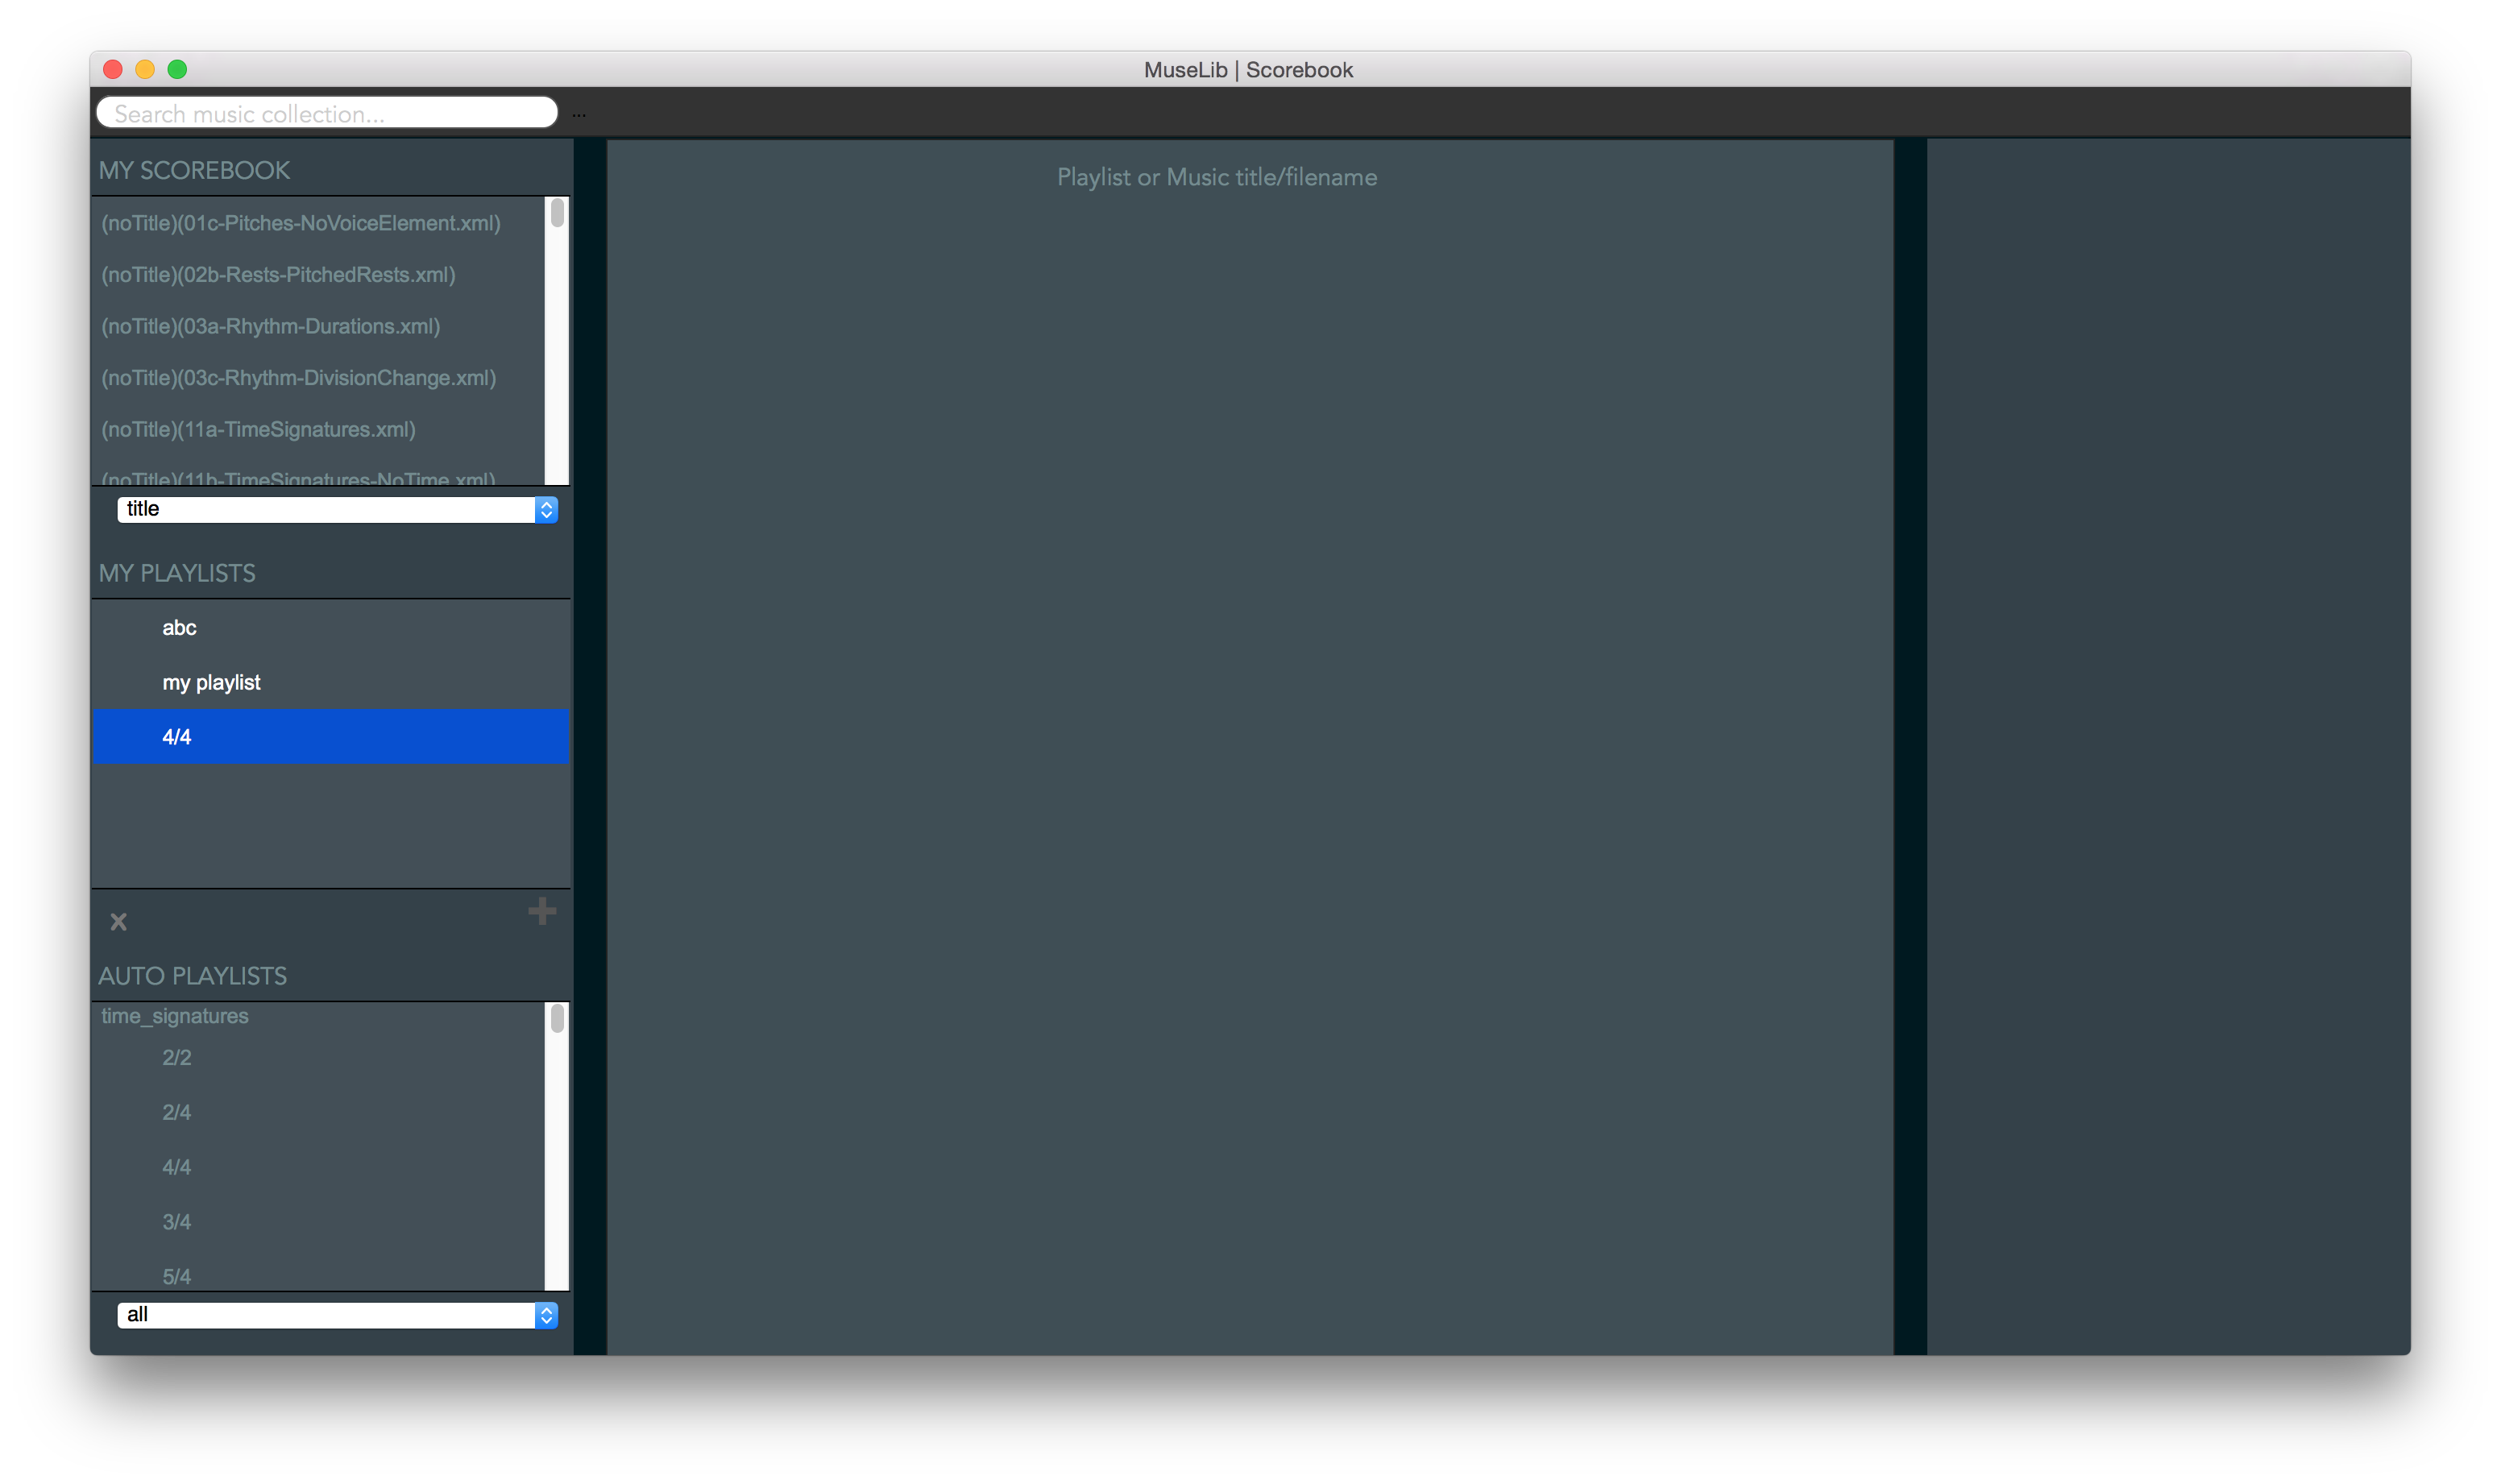
\includegraphics[width=400pt]{main_dark}
\caption{The dark theme}
\label{fig:theme2}	
\end{figure}

\begin{figure}[H]
\centering
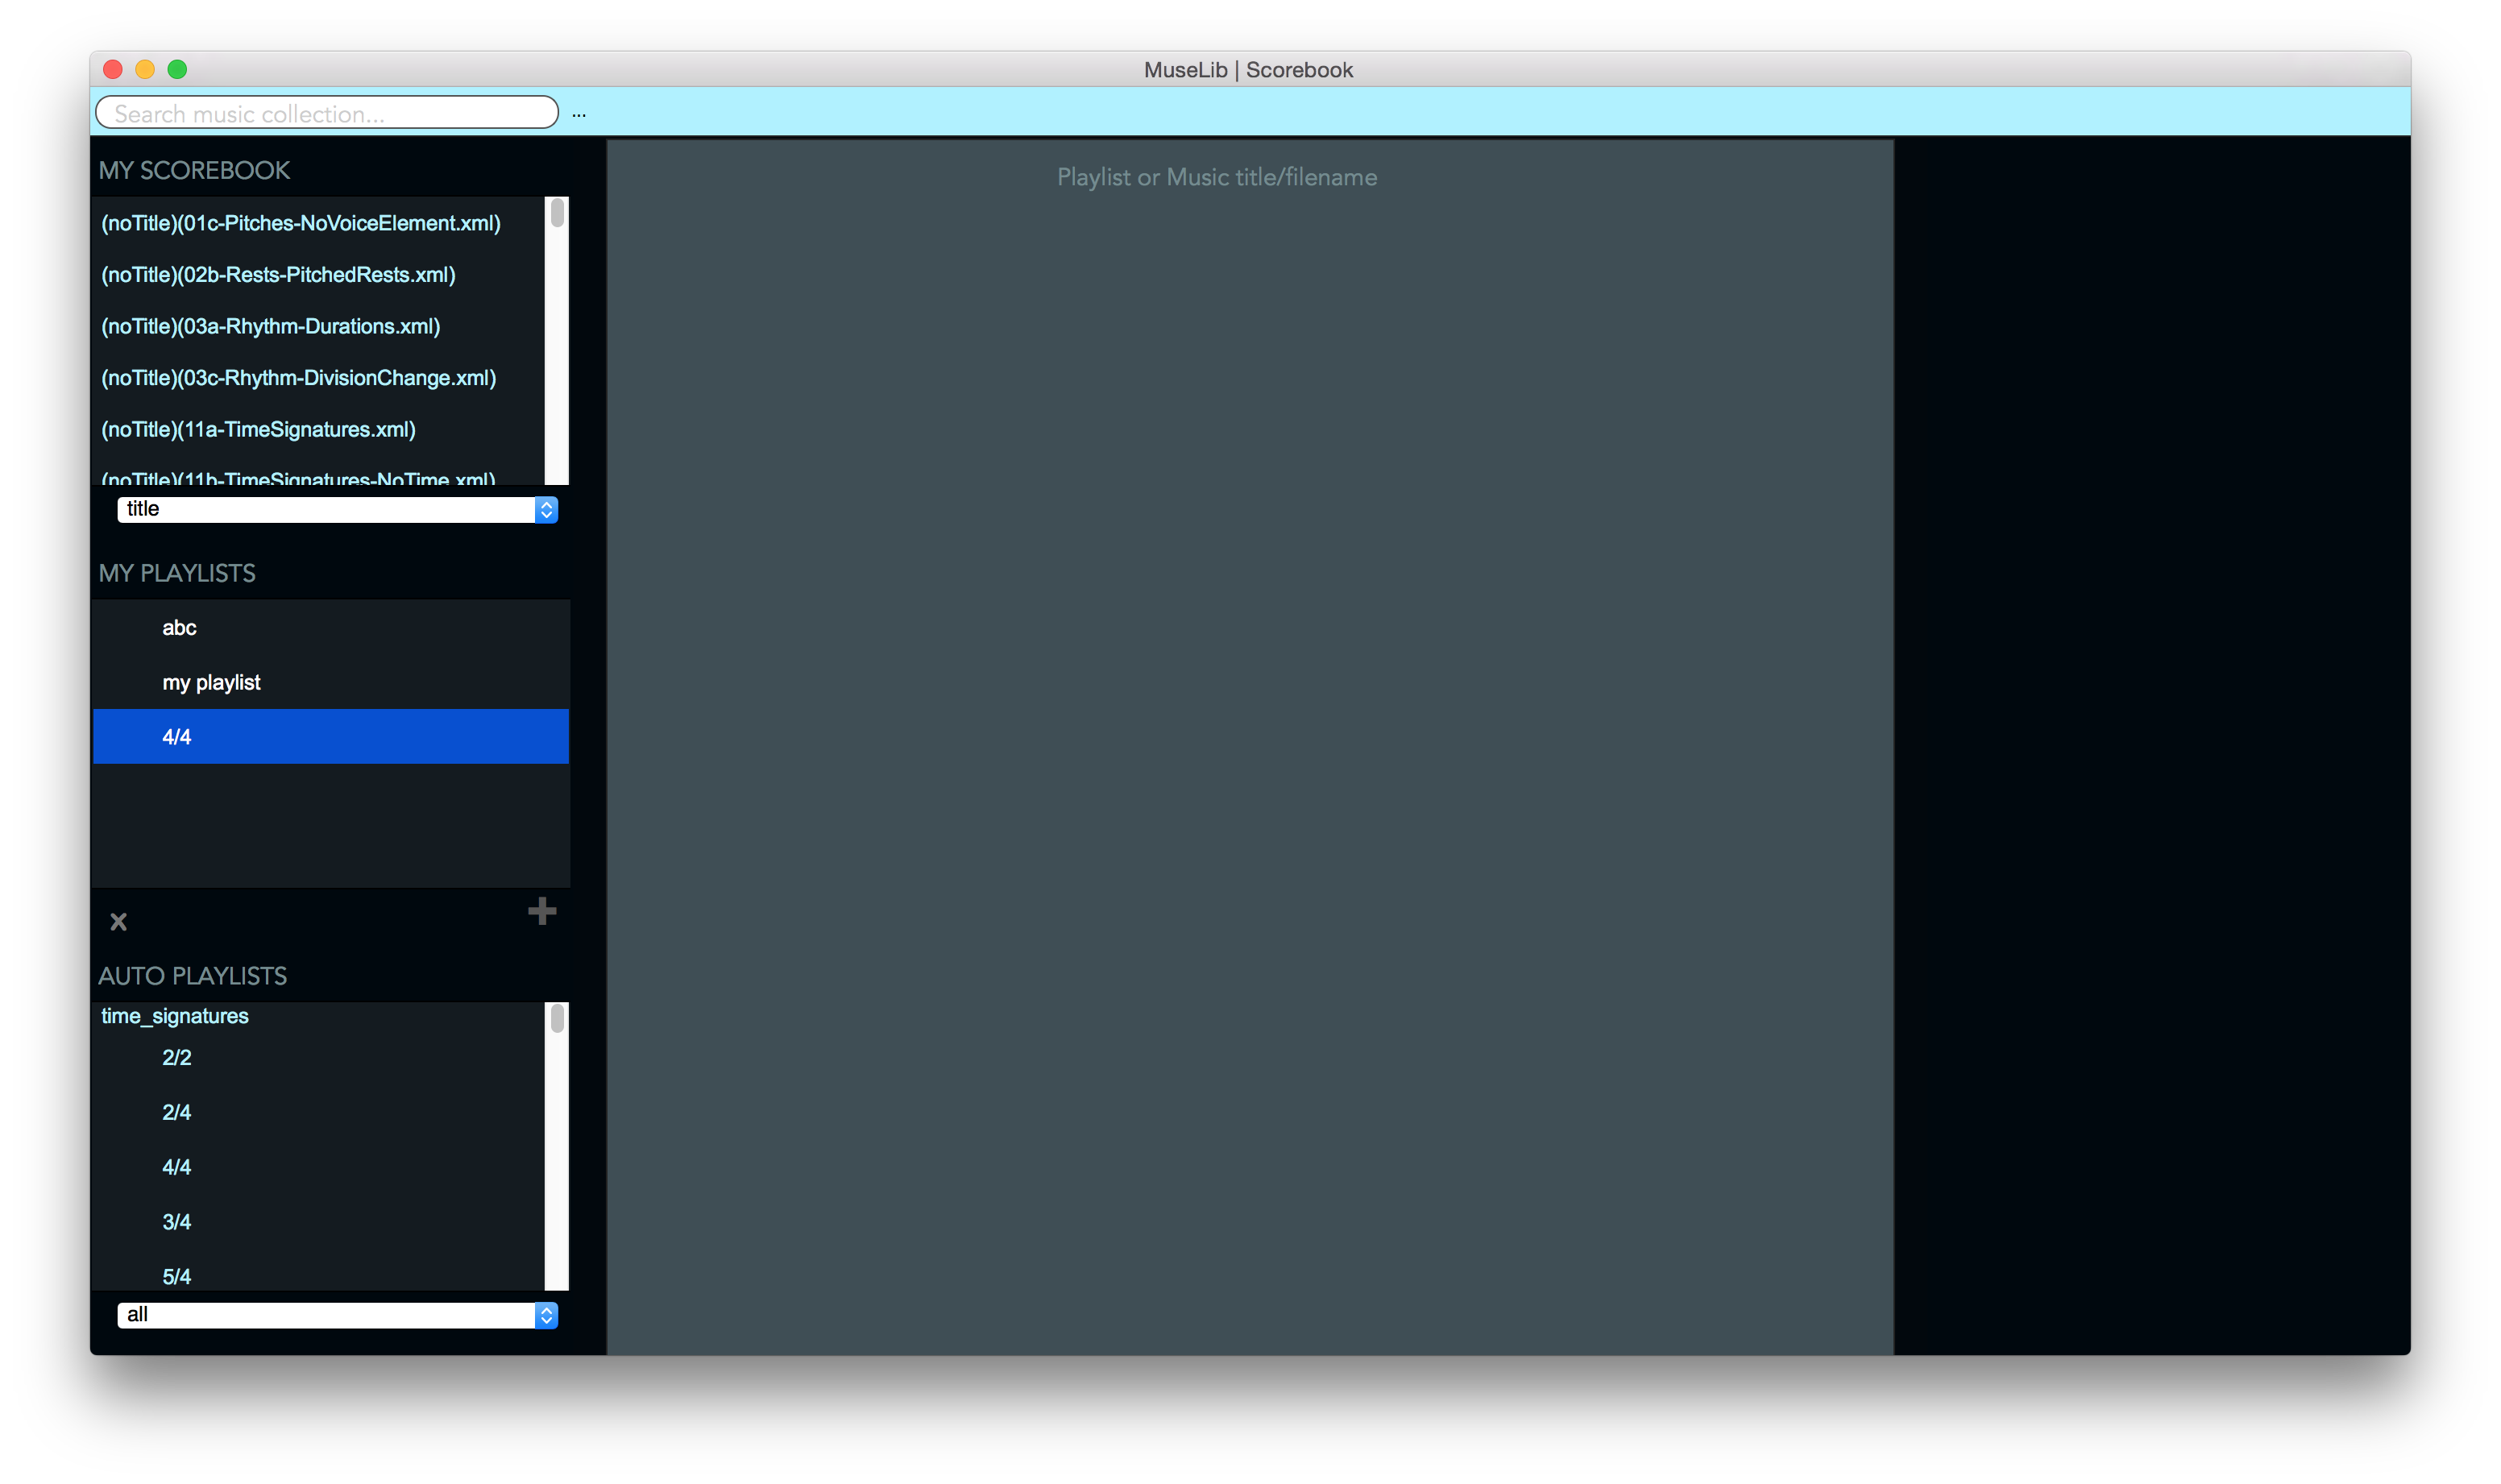
\includegraphics[width=400pt]{main_electric}
\caption{The electric blue theme}
\label{fig:theme3}	
\end{figure}

\begin{figure}[H]
\centering
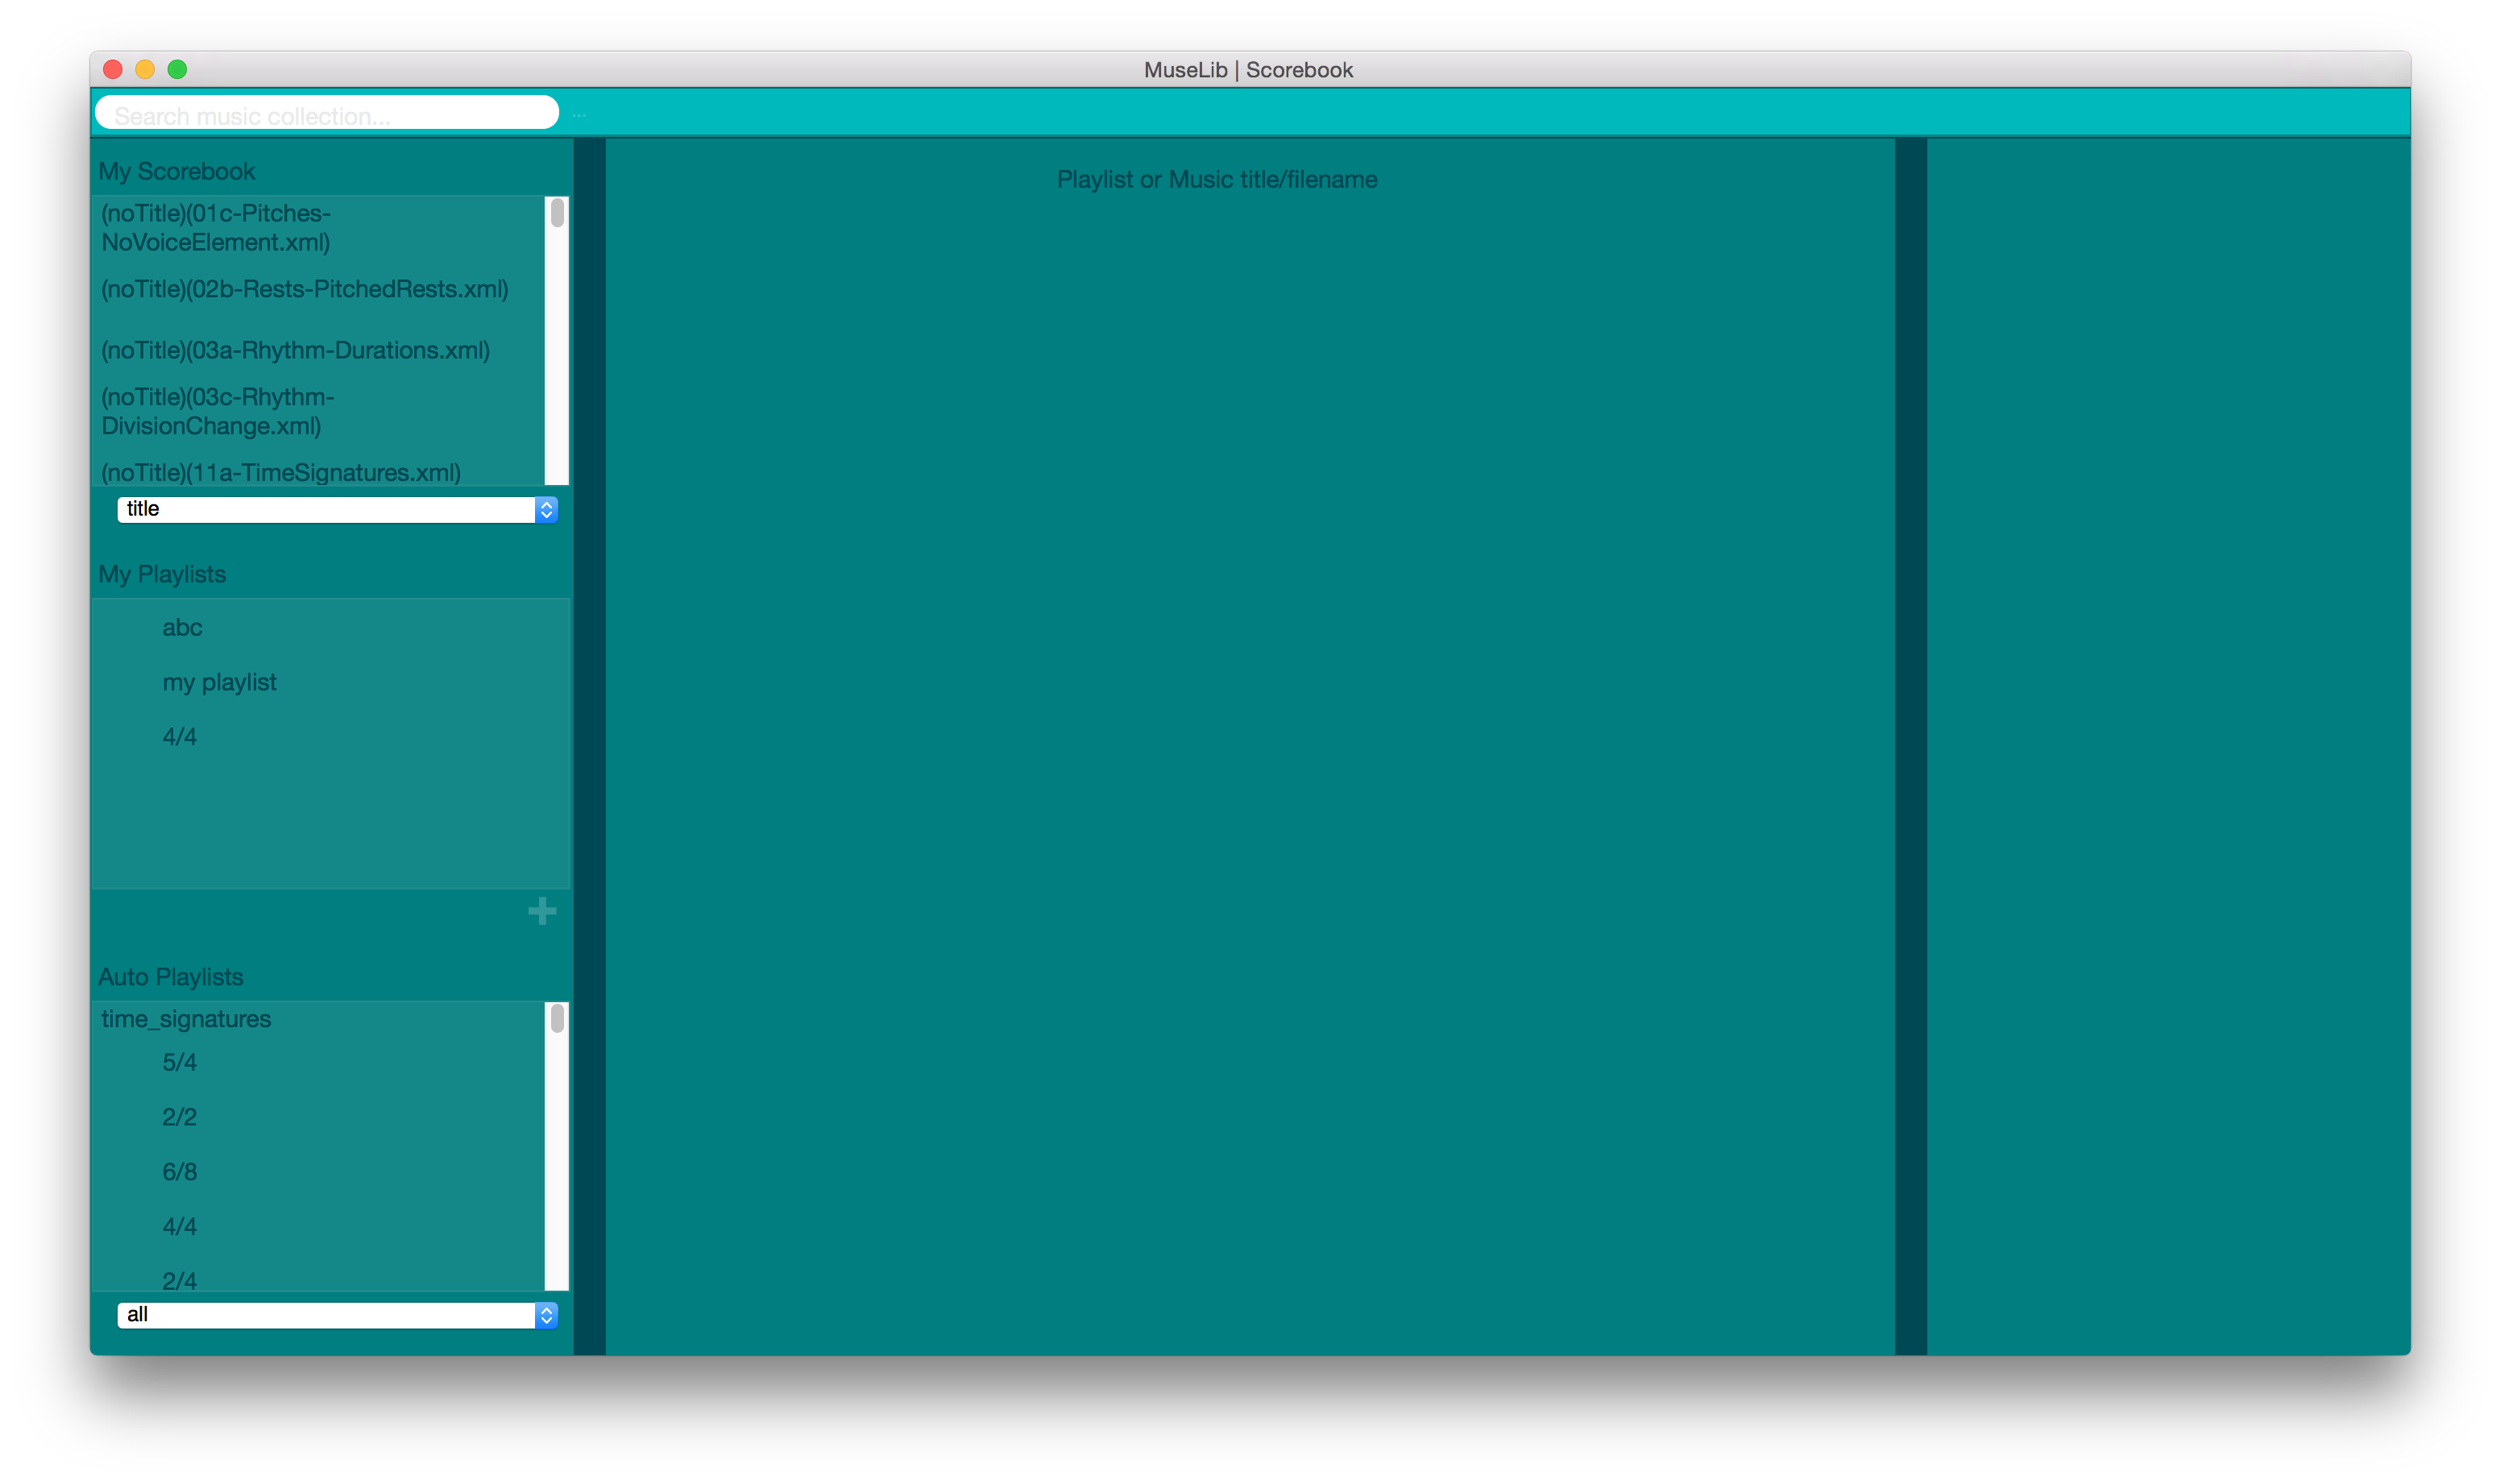
\includegraphics[width=400pt]{teal}
\caption{The teal theme}
\label{fig:theme4}	
\end{figure}

\subsubsection{Customising your widget views}
Any and all of the widgets to the right and left of the main pane can be hidden or displayed using the View menu, as shown in figure \ref{fig:view}.

\begin{figure}[H]
\centering
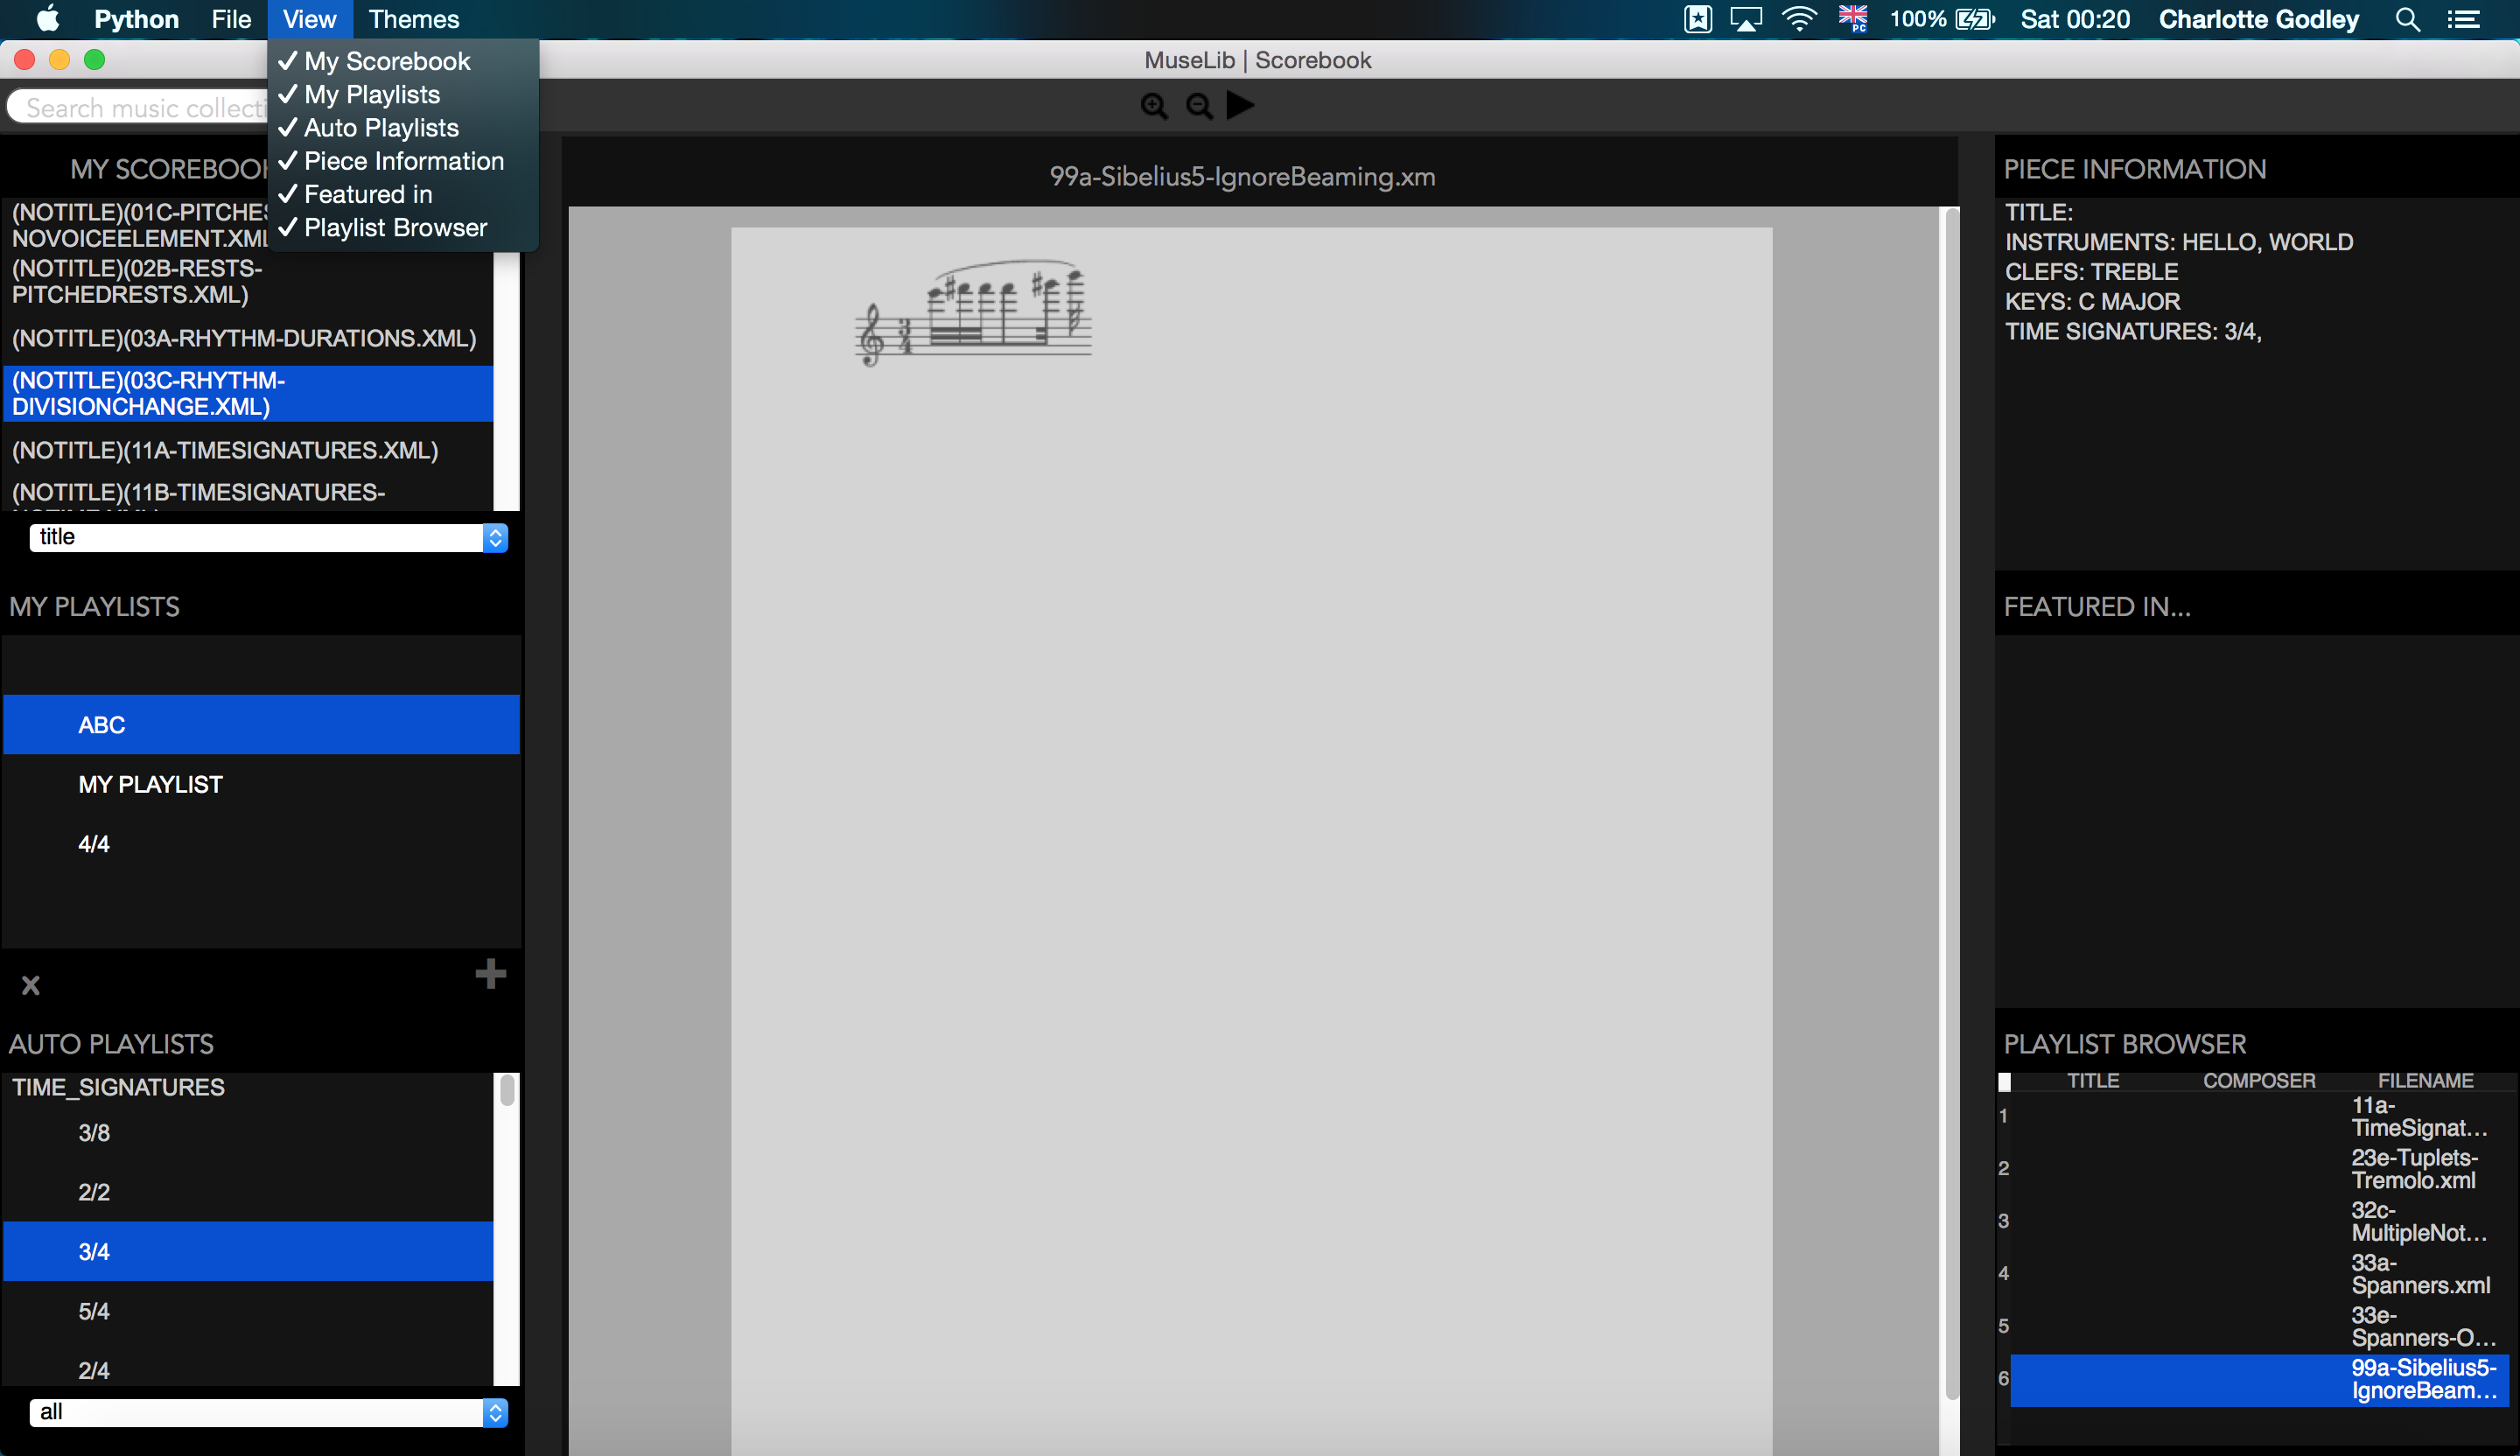
\includegraphics[width=500pt]{view}
\caption{The view menu}
\label{fig:view}	
\end{figure}



\section{Background}
\subsection{Problem Context}
This problem's main focus is the difficulty of organising classical sheet music, and how this can be made easier by the automatic extraction of key pieces  of information. In order to understand what a performer may want to know about a particular piece, it is important to have a brief understanding of the elements of musical notation common to all compositions.

The key element of this form of notation is the staff, as shown in figure \ref{fig:staff}. This is a grouping of five horizontal lines, with each line or space in the staff indicating a different sound pitch, a term meaning the relative "highness" or "lowness" of the sound \parencite{classroom}.

\begin{figure}[h]
    \centering
        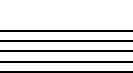
\includegraphics{staff-crop.pdf}
    \caption{A blank staff}
    \label{fig:staff}
\end{figure}

This staff is divided by bar lines, vertical lines delineating grouped units of sound and silence (formally referred to as notes and rests), which provides an indication of the unit's relationship in time by its juxtaposition to other groupings in the composition. These groupings are called measures or bars, with each bar having a variable maximum of notes and rests. 

\begin{figure}[h]
    \centering
        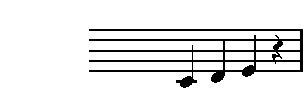
\includegraphics{bar_with_notes-crop.pdf}
    \caption{A bar containing three notes and one rest}
    \label{fig:staff-notes}
\end{figure}
\subsubsection{Clefs}
In the system of staff notation, sound frequencies, or pitches, are denoted by letters A-G - after each cycle of the letter names, the next pitch above it will be the start of a new cycle. The cycles are often split by octaves, a term meaning eight pitches, for example A to A or E to E. 

In order to provide a link between the lines and spaces of a staff and pitch name, a clef symbol is necessary.
\begin{figure}[h]
    \centering
        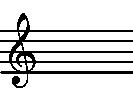
\includegraphics{clef-crop.pdf}
    \caption{A staff with a treble clef}
    \label{fig:clef}
\end{figure}

Each clef symbol denotes a different pitch name - figure \ref{fig:clef} shows a G. The center around which this symbol is drawn - in figure \ref{fig:clef}, the second line from the bottom of the staff - indicates that this line or space will be known as the pitch name denoted by the symbol. From this the reader can infer all other pitches by counting through the letters of the cyclic octave system, so in figure \ref{fig:clef}, the space above becomes an A, and the space below becomes an F.

This symbol is important to a musician as different clefs are used to position the majority of the pitches in a piece on the staff, as this makes it easier to read. From this a performer can infer the average range of a piece, and predict whether this will be comfortable for the performer's chosen instrument or voice.

\subsubsection{Keys}
A second important indication to the player is the key, denoted by a key signature.
\begin{figure}[h]
    \centering
        
\includegraphics{key-crop.pdf}
    \caption{A staff with a key signature}
    \label{fig:key}
\end{figure}

The key signature is a collection of symbols at the beginning of the piece which indicate which pitches should be raised by half pitches, and which should be lowered. Raised pitches are called sharps, indicated by the \# symbol, whilst lowered pitches are called flats, indicated by the $\flat$ symbol. Each key, which has a letter name and key type (which can either be "major" or "minor"), has a different combination of flats or sharps. 

This is a useful piece of notation to a musician as pieces in less common keys, such as C\# major or F\# major, may prove more difficult for the user to perform, and therefore they may want to filter out pieces in these particular keys. Similarly, in the case of singers, a singer's range may sit comfortably in one or two keys and they would perhaps want to find pieces in only these keys. 

\subsubsection{Meter}
The third symbol denoted at the beginning of a measure is the meter or time signature, displayed as two numerals positioned like a mathematical fraction.

\begin{figure}[h]
    \centering
        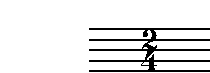
\includegraphics{meter-crop.pdf}
    \caption{A staff with a 2/4 time signature, or meter}
    \label{fig:meter}
\end{figure}

The upper number of a meter symbol indicates the amount of beats in the bar. A beat simply refers to a note or rest, and the type of beat is indicated by the lower number. In the case of figure \ref{fig:meter}, 2/4 indicates a measure will contain 2 crotchets, or quarter-length notes. The most common time signature is 4/4, which for this reason is usually denoted with a C in place of the fraction, meaning "Common time".

This information is important as it tells the performer how the rhythm and beat of the piece should be felt, counted and performed, and is useful for searching purposes as different meters give the piece a different feeling, dictating the sort of occasion this piece would accompany. 

For example, 2/4 is commonly used for march pieces, and 3/4 is commonly used for waltzes and dance pieces.

\subsubsection{Tempo}
The speed of a particular piece, or the tempo, is indicated by an equation.

\begin{figure}[h]
    \centering
        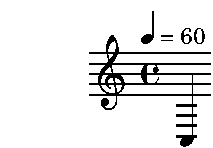
\includegraphics{tempo-crop.pdf}
    \caption{A staff with tempo marking}
    \label{fig:tempo}
\end{figure}

The equation above the staff in figure \ref{fig:tempo} indicates that the piece should be played at 60 beats per minute. The symbol dictating the sort of beat per minute depends on the time signature, here a crotchet (or quarter note) is given as the piece is in 4/4 time. Sometimes, this will be accompanied by a text direction to indicate speed or style, such as Andante, indicating a walking speed.

This indication would prove a useful identifier as pieces of different tempos provide variation in performance lists, so a concert organiser may want to find pieces with a variety of tempos.

\subsubsection{Further metadata}
Aside from these symbols, there are some items of textual information useful to the user. 

The first of these would be the parts in the piece and their transpositions. A part refers to a grouping of measures given to one performer, as shown in figure \ref{fig:parts}. "Part" used in a general sense usually refers to the names given to the left, in this example, "Clarinet in B$\flat$" and "Flute".
\begin{figure}[H]
\centering
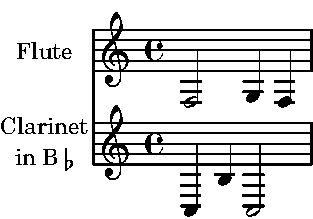
\includegraphics{multiparts-crop}
\caption{Two separate parts in one score}
\label{fig:parts}	
\end{figure}



Parts would be relevant as a particular group of instrumentalists may need parts that fit their instruments. If this is not the case for a given piece, however, a part written for a different instrument, for example, the Alto Saxophone rather than the Tenor Horn, may be compatible with the instrument anyway, if the transposition matches the instruments together. 

An instrument which has a transposition means that, whilst most instruments would play a note as it is written, a transposing instrument will automatically sound the note in a different key, as described earlier, which may raise or lower the sound of the note. For example, the note C played on an Alto Saxophone will sound as an E$\flat$, because it is in the key of E$\flat$ major. 

Further to this, the user would want to know the piece's title, and names of publishers, composers, arrangers and lyricists of the work, commonly known as the bibliography of a piece\parencite{MIR}. Further to the composer name, it may be useful to know the date of composition as an indication of the era in which the piece was composed, such as Classical/Baroque/Romantic, though this would not always be written on the sheet music so may need to be researched using the Internet.

\subsection{Comparison of Technologies}
\subsubsection{Programming Language}
This project could be developed with a variety of programming languages, as displayed in table \ref{table:langs}.

\begin{table}[H]
\centering
\begin{tabular}{| l | l | l | l |} \hline
  {Language} & {Speed of development} & {Developer's Knowledge} & {Most recent use} \\ \hline
  C\# & Fast & A lot & 2nd year \\ \hline
  Python & Fast & A lot & In constant use for over a year \\ \hline
  C++ & Slow & Average & 2nd year \\ \hline
\end{tabular}
\caption{Table of languages considered}
\label{table:langs}
\end{table}
The first language in consideration is C#. C# is mostly used on Windows due to the main compiler being closed source, but with some platform independence due to the Mono Project, which is feature-complete to C\# 10 \parencite{MonoDev}, or Xamarin Studio and other such tools, but the developer has not developed any applications with C\# for use on multiple operating systems. 

In terms of speed of development, the developer considers that the language syntax is reasonably intuitive and consistent, but that by virtue of the language being statically typed, considerations such as dynamic typing and the need to write more code in terms of key strokes, the second language consideration has the advantage.

Finally, due to the language being mostly for Windows and largely being closed, C# has a lower amount of Open Source projects on the popular Open Source Code Repository Github, as shown by the graph in figure \ref{fig:graph}. Whilst this is not necessarily important to development at this stage, the developer intends to Open Source the project and if there are more repositories for Python, as the graph indicates, this would potentially mean there would be more potential contributors.

\begin{figure}[h]
\centering
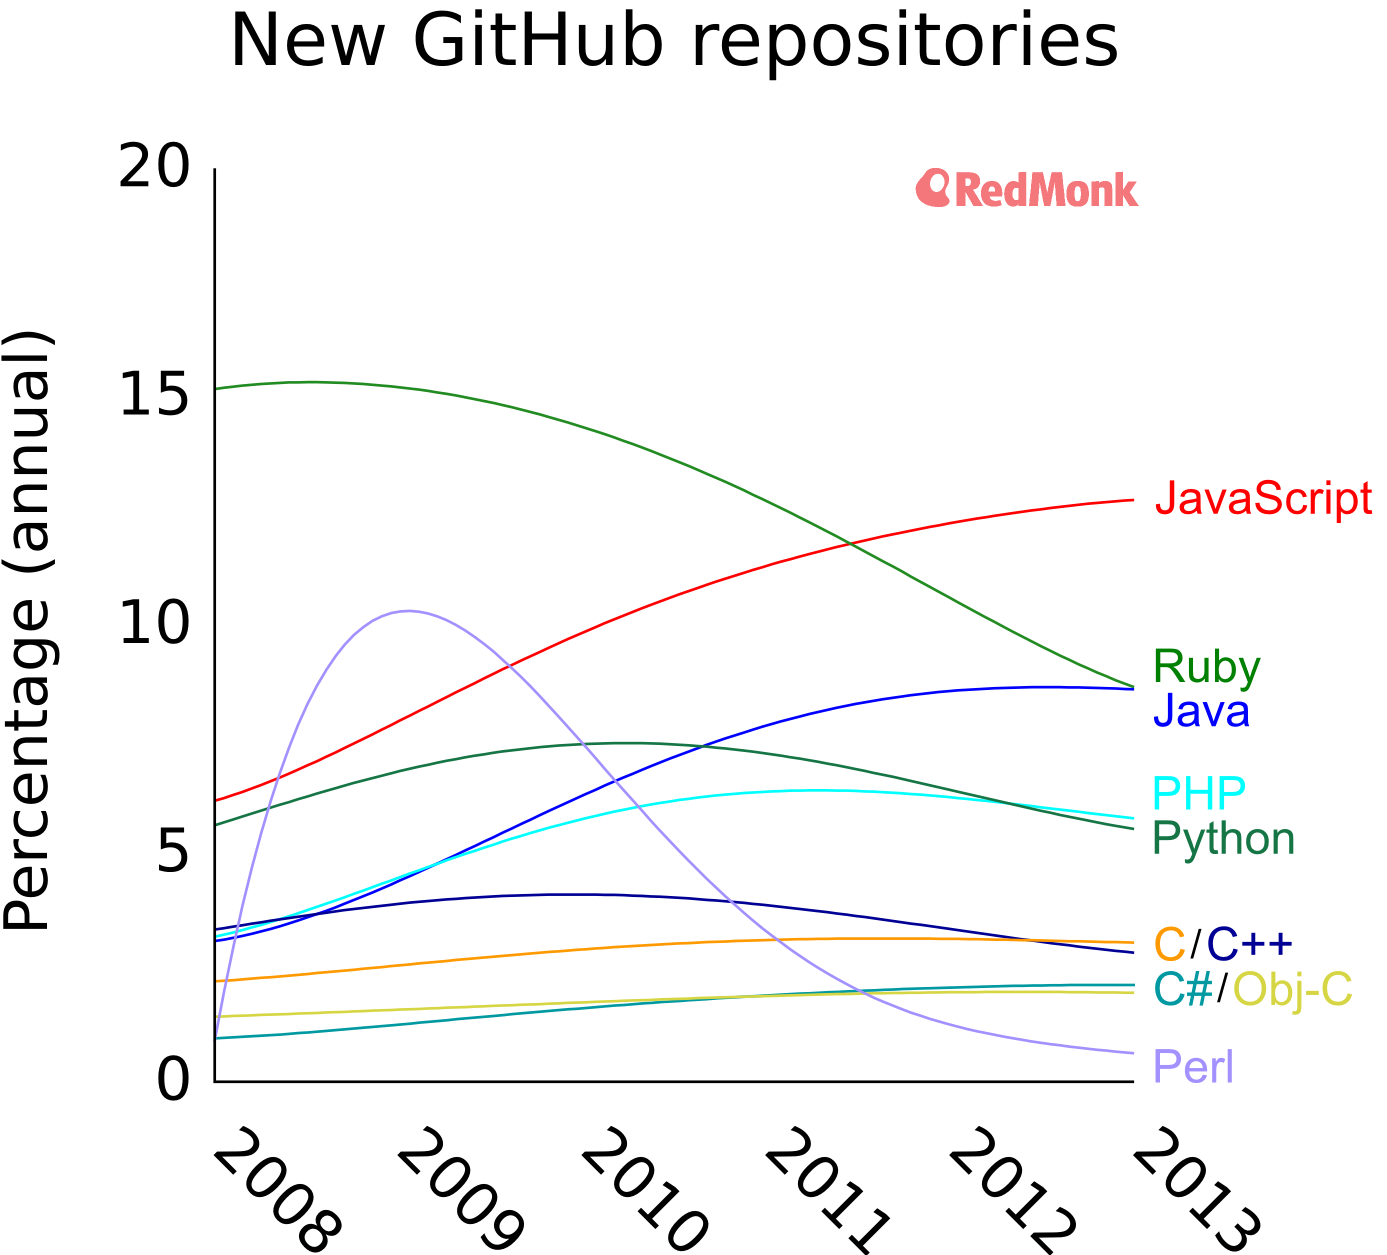
\includegraphics[width=250pt]{github-repos}
\caption{A graph showing the percentage of repositories on Github in different languages}	
\label{fig:graph}
\end{figure}

The second language in consideration is Python. Python is cross platform, as it is included by default in OSX and Linux based Operating Systems with the ability to install it on a Windows operating system.

In terms of development speed and syntax, Python's syntax is the closest of the three considerations to english or pseudocode, and thus requires the least amount of key strokes. Being closer to english also means that the project is more likely to attract a wealth of less technical contributors, in particular musicians, as the language should be easier to learn how to use.

 Furthermore, as it is dynamically typed this allows the developer to use a particular advantage of ducktyping whilst developing, meaning that so long as a class has a particular behaviour, the program can use the class for it's purposes and ignore differences to other classes without implementing an interface.
 
 Lastly, there are many current projects written in Python in the area of Music research \parencite{pmus}, which means the project will be easier to integrate and communicate with other projects or build upon the work of others without needing to port software to Python.

The third and final language in consideration is C++. Whilst C++ is arguably the closest to native code and therefore the language which will be the best for cross platform development, the syntax and memory management issues of C++ mean that development can be slower, particularly when the developer does not feel as competent using this language.

It is for these reasons that Python has been chosen as the development language. Beyond the selection of Python, it is important to discuss and consider which version to use, as Python 3 was introduced in 2008, but Python 2 continues to be maintained and was updated to include many of the backwards compatible features in 2010. Whilst this seems an obvious choice as Python 3 is the latest version, many projects still have issues updating and using Python 3 as it was deliberately not backwards compatible \parencite{Foundation2}.

Upon due consideration, Python 3 has been selected, though if the project requires legacy libraries this may have to be evaluated again. This decision has been made because at this stage the project does not appear to require libraries which do not work with Python 3, and therefore the developer should make every effort to keep the project up to date with the latest version.

\subsubsection{File format}
The project will require at least one default format for it to process music, which needs to have detailed information about what the score contains. Table \ref{table:formats} describes the options considered.

\begin{table}[H]
\centering
\begin{tabular}{| c | c | } \hline
  {\textbf{Format}} & {\textbf{Purpose}} \\ \hline
  muscx & MuseScore notation \\ \hline
  SIB & Sibelius notation \\ \hline
  new format & this project only \\ \hline
  MusicXML & sharing music between software \\ \hline
\end{tabular}
\caption{A table showing the different file formats considered}
\label{table:formats}
\end{table}
The first two options, muscx and SIB files, are formats used by the open source notation software MuseScore \parencite{MuseTour}, and the world's most popular proprietary notation software, Sibelius \parencite{avid}. Using either or both of these files would mean the majority of users would be able to use the application. 
However, both options couple this project with those particular packages, when users could still choose other software to write music with. Furthermore, the formats are specifically designed for those software packages and may have nuances which make development for this project more difficult. Additionally, Sibelius is proprietary so borrowing their file format may cause copyright issues.

The third option is to create an entirely new format. This would mean the file format was designed to the requirements of the project and therefore be entirely customisable and extensible. However, this project is created with the intention of organising, not composing music, so the project would also need to produce a converter from other file formats which is not desirable.

The fourth and final option is MusicXML, a file format intended for sharing and archiving the world's sheet music \parencite{mxml}. This particular format is used by a wide variety of software packages \parencite{mxml} and is included in the formats usable by both MuseScore \parencite{MuseTour} and Sibelius \parencite{avid}, therefore neither couples the format with a program nor requires manual creation and import of current music files. 

Aligning the project with an open format like this will make the project a better renderer, as the project will be designed to handle MusicXML more effectively than other packages which are designed to use their own format by default, then import or export to MusicXML, such as MuseScore \parencite{mscoreBugTracker}.

However, this particular format was designed by a third party, Make Music, who have a vested interest in the file format and it's structure as they produce Finale, another popular music editing package\parencite{mxmlSoft}. This means that the design aims of the file format have a particular alignment to that platform, and will not necessarily be logical to work with.

Using MusicXML also means that there will be a technical challenge of learning how to use and understand MusicXML, which may affect the development time adversely if the developer does not pick up enough initial knowledge to design the system effectively.

For reason of inclusion in composition software packages, MusicXML has been selected as the file format for the project. 

\subsection{Comparison of Algorithms for Rendering Music}
Figure \ref{fig:flow} shows a flow diagram for the system of rendering sheet music. Each decision taken in order to reach this method will be discussed in detail below.
\begin{figure}[H]
    \centering
    \includegraphics[width=80pt]{render_algorithm-crop}
    \caption{A flow diagram describing the rendering system}
    \label{fig:flow}
\end{figure}

\subsubsection{Algorithms for parsing XML to memory}
For the rendering of sheet music, the system must in some way manipulate an XML file to an output format.

The first option for this would be applying an XSL stylesheet, which is commonly the method of choice for rendering XML files in a web browser. This is not an option in MusicXML because the notation is too complicated and requires too many symbols, whilst XSL stylesheets are usually used for images and text representations. Sheet music is somewhere in between the two, and thus this option cannot be selected.

The second option would be to create or reuse a converter script from XML to the output format, meaning the output would be generated at the same time as the input. However, this couples the system with MusicXML and would slow down development if it were required to use a different additional input, or decisions were made to change the output format. Furthermore, the Big O representation of this type of script to any output format is $O(n^2)$, whilst the selected final option using objects would be $O(n)$.

The final option, which has been chosen for the project, is to create a converter script which would parse the MusicXML and create a hierarchy of objects. This avoids coupling directly to MusicXML as new formats of both input and output would only need a converter script creating to the object hierarchy which would then handle input or output to other formats.

However, whilst this avoids coupling, a technical challenge is created using this method in that the object structure needs careful planning to cater for the structure of MusicXML and the structure or method of output, which with little knowledge of the input or output format is difficult to achieve.

\subsubsection{Rendering Algorithm}
The program is required to take the object structure and transform it, in some way, to readable sheet music. The user should be able to pan around the sheet music and zoom in and out of it to view specific details.

This could be achieved using an entirely new algorithm, with the output going directly to the render window using different glyphs and fonts extracted from their relevant classes.

However, the functionality of panning and zooming using this algorithm may be difficult to optimise, as both could possibly require running the algorithm each time the user provides input. 

Furthermore, the conversion of even basic sheet music to a readable format would require a high level of precision and complexity, and creating a new algorithm would be considered reinventing the wheel, so to speak, as this is a process that has been covered by many different applications (like MuseScore \parencite{MuseTour}, Finale \parencite{mxml} and Sibelius \parencite{avid}). 
Lastly, the process of debugging whether the symbols are correct would require visual checking and would be difficult to debug automatically.

It would be possible to alleviate the panning and zooming problem by converting the collection of symbols to an image or PDF file and using a built in image rendering library, such as wxPython \parencite{WX}. However, this method still involves reinventing the wheel and incurs problems with visual debugging.

Considering these factors, it has been decided that the algorithm will be outputting files to a third party system known as Lilypond. Lilypond is a language and system developed to typeset the highest quality sheet music \parencite{Lilypond}, which takes an input file and outputs a PDF or image. As this is a language unto itself and has been in development for many years by the Open Source community, this will alleviate the problem of visual debugging - instead, each class can create a formatted Lilypond output based on its attributes and unit tests can automatically confirm that the result is as expected.

\subsubsection{Algorithms for parsing XML for information}
For the parsing of XML itself, there are two potential built in methods to choose from. The first, known as DOM or Document Object Model, loads the entire XML file into memory and provides methods to search the loaded file for specified tags. The developer has used this before in personal and industrial projects, and believes it is cumbersome to manipulate data in this way. Furthermore, this project is focussing on rendering the information rather than rendering it with precise formatting, and many software packages implant musicXML files with very complex formatting information which may or may not be necessary\parencite{MusicXMLPresentation}.

The second option is using a different api called the Simple API for XML (SAX). In this method, the program loads the XML file tag by tag, and connects to call backs when specified things occur in the file, for example a new tag or piece of data inside tags, or the closing of an old tag. This is easier to work with as functionality can iteratively be built up by creating handlers for each tag, and is better for memory management as only tags which are necessary to the project will have any effect on the object structure. For these reasons, this method has been selected.

\subsubsection{XML verification algorithm}
For both the algorithm options discussed in section 3.3.1, a further choice is whether to verify the XML parsed, using an online file validator, or presume the file is written in valid MusicXML. 

The usual choice is to verify all XML, and is therefore the default option for both methods of parsing. Whilst this confirms that XML is valid before starting parsing of a file which could be corrupt, the speed at which files will parse is greatly reduced according to the speed of the user's internet connection.
Furthermore, if the user is browsing their own music collection, it should not be necessary for the user to be connected to the internet.

Due to speed and functionality considerations, the choice has been made that the XML parser algorithm will not verify XML being converted to objects, or being examined for metadata. Given that most musicXML will be produced automatically by other programs, it is unlikely files opened by the project will be corrupt, though necessary steps will be taken to avoid this causing a problem in the program.

\subsection{Comparison of Algorithms for Organising Sheet Music}
The system design for the automatic extraction of meta information for each sheet music file is described by the flow diagram in figure \ref{fig:meta}. 
\begin{figure}[H]
    \centering
    \includegraphics[width=250pt]{metadata_algorithm-crop}
    \caption{A flow diagram describing the meta scanning system}
    \label{fig:meta}
\end{figure}

Figure \ref{fig:uiLoader} shows how the user interface will load the information and apply the rendering algorithm. Finally, figure \ref{fig:metaSearching} shows how search and autocomplete will function. The decisions made in order to arrive at these methods shall be discussed and compared in the following subsections.
\begin{figure}[H]
    \centering
    \includegraphics[width=250pt]{UI_loading_algorithm-crop}
    \caption{A flow diagram describing the loading of metadata and usage in the User Interface}
    \label{fig:uiLoader}
\end{figure}
\begin{figure}[H]
    \centering
    \includegraphics[width=250pt]{search_algorithm-crop}
    \caption{A flow diagram describing the loading of metadata and usage in the User Interface}
    \label{fig:metaSearching}
\end{figure}
\subsubsection{Metadata Model}
In order for the system to scan a file for data, a model of what data to collect will need to be designed and implemented. In normal circumstances there may be a model already described as standard for the subject area. In the case of music and music research, there are many facets and disciplines which have an interest in collecting data about music \parencite{MIR}. For example, a musicologist may want to study patterns, a sound engineer may want to study instrument timbres and transpositions, or an Artificial Intelligence researcher may want to study the generation of music in a general sense \parencite{creativeMachines}. 

For these reasons, there does not appear to be a standard model, and therefore this project will create a new, general model for music information retrieval.
There are two options in consideration for the model of data to collect.

The first is to collect general symbolic data, such as the elements described in the problem context - time signature, meter, clef, key, instruments, transpositions, and bibliography information. This provides data that will be useful to every musician reading the music, gives a reasonable amount of complexity and variation and allows for a wide range of searches.
However, this does not provide many specifics to instruments, as for example, a piece containing a lot of pitch movement or certain sequences of notes may prove difficult to one instrumentalist, but not to another. 
Furthermore, for the difficulty scanner objective this model would need to be expanded to include note durations and patterns, and apply some semantics to the model to deduce the grading.

The second would collect data with specifics according to instrument name, and make the parser apply certain rules to deduce what would be useful for each player to know. This provides more precision to the data and has a higher likelihood of being useful data to the user. 

However, this would be more technically challenging due to the need for semantics and specific structuring of data in a way that the first option would not, as the data has a lot more variance from piece to piece and part to part. 

Additionally, relying on the instrument name to deduce rules to apply may be a problem due to different spellings of names which would mean the scanner would have to prepare for all possible changes (for example some pieces may use plurals to indicate more than 1 instrument should play 1 part, and some pieces may provide the key as well as the instrument or some may use the default which the scanner would have to deduce, like "Clarinet" or "Clarinet in Bb"), and also have to handle language as different human languages use different instrument names, like Klarinette in German.

The developer has decided to use the first option, but design the system so that the parser could be expanded at a later stage of development to allow for difficulty ratings and other usecases.

\subsubsection{Memory considerations}
The metadata algorithm has been designed so that, for a given folder, the program will parse all of the files with the XML extension for the model described in the previous section. It will be necessary in some way to store this information, potentially both physically to avoid unnecessary repeat meta data scans, and in memory to allow the program to manipulate the data.

It would therefore be possible to simply extract the data and store it to an in memory object, which would then be loaded and saved to a serialised python object file. This would be quick to develop as it only requires using the Python serialisation libraries in collaboration with the XML acquisition libraries, and has a simple system design. 
However, the algorithms and overall design of the memory object would mimic much of the functionality of a database, so would be considered duplication of other people's work with little technical improvement. 
Furthermore, any extensions other developers made to improve or change the dataset would have to be written or connect to Python, as this would be the only way to unserialise and understand the outputted file.

The chosen solution therefore is to extract data, then communicate with a database instead of an in memory object. Queries to the database would result in ordered lists of files and tuple data sets which could then be manipulated by the system. 

This is preferable to the earlier suggestion because database systems have been worked on by multiple contributors(ref)%TODO: REF
 and are designed to be faster than many searching and sorting algorithms by virtue of a B-Tree file structure \parencite{SQLiteBTree}. For these reasons using a database would most likely have faster access and search times than an in memory object.

Furthermore, using a database avoids coupling any future improvements to Python, as the most common database structures have well designed APIs for the most popular languages. (ref)
% TODO: REF

\subsubsection{XML data acquisition algorithm}
The system should take in a selection of XML files and parse them for information. As described previously, this could use either the DOM method of XML parsing, or the SAX method of parsing.
The system will use SAX because there are only a select few tags and collections of information that the database will need to peruse, and SAX means that only these tags will have an effect on the algorithm or memory.

\subsubsection{Query Processing Considerations}
The application should allow the user to input a search query and find results which match the input. A user can then select from a list of result options which will render the selected file. In order to deduce what tables and data sets to query based on user input, it will be necessary to structure the query in a certain way.

The first option for achieving this would be to define a querying syntax and provide the user with instructions or a tutorial on how to use this syntax. This allows for a lot of complexity and means that the program will not need to do as much string manipulation and processing.

However, this also makes the program less intuitive to use and could cause users, particularly those who are less technical, to be confused or apathetic to the program if the syntax is too complicated. Furthermore, some searches, such as finding all pieces by Mozart, do not require a high level of complexity as these are merely textual input.

Another option would be to allow the user to input anything and try to predict from the input which table to query. This would easily be achievable for text input and for input which has symbols specific to one notation element or another. An example of this would be a time signature, which is the only input which would be represented as a fraction, like 4/4, or perhaps a tempo indication as it would always have an equals symbol in the input.
However, this removes the ability to build up complex queries and for some elements, like clef or key, it would not be possible to deduce merely from text what the user is expecting. This could potentially result in the system querying all tables for the data, or result in excluding some elements of meta data in order to avoid a processing overhead.

The selected option therefore will be an amalgamation of the two described options, which will allow for both simple strings, such as 4/4 or quarter=half when defining time signatures and tempos, and for more complex input, such as instrument:clarinet with:clef:alto. This will enable users to search without needing to know or use too much search syntax and is aimed to be intuitive and simple. Instructions for the querying syntax will be provided in the user guide in the appendices.



\subsection{Comparison of Technologies for Importing Online Musical Sources}
\subsubsection{Musical Sources}
The project should be able to communicate with one or more online music catalogs in order to allow the user to expand their collection. Whilst the system should be designed for extendability, at least one source should be integrated to the system to prove functionality.

The source this project focusses on using is \textbf{MuseScore Online}, which is a community website created for composers to upload, share and discover compositions using the MuseScore platform \parencite{MuseShare}.

This has been selected due to the number of files available, the openness of the platform and the well documented API. It will, however, be necessary to manage copyright issues, as pieces published on this website may be published under the license of the composer's choosing and therefore may cause issues with certain types of users, in particular those performing commercially.

\subsubsection{Searching Algorithm}
The APIs for the selected source provides a certain amount of bibliographic information at each piece when queried. The algorithm for searching this data will need to collect and parse data from the API, and allow the user to search this data in order to download relevant files.

The first option for achieving this would be to search the API using only bibliography information whenever a user enters a query containing requests for bibliography, provide the options to the user then download the file if needed. This would be simple to implement, however it would be slow due to needing repeated connection to the internet. It would also cause an overhead on the server side because of this repeated connection, and users would not be able to search online collections using the advanced methods described in section 3.4.4. 

It has therefore been decided that the system will collect all the data from the server about every piece in the catalog, extract the bibliography information for use later, then download and parse each file for meta data, combine that with the bibliography information and finally, put the data into the database and then delete the XML file. 

This would mean the data collected would be the same quality and quantity as locally stored files, and can be searched using the same level of complexity. It also avoids the issue of repeated connections to the API, as this would only require a connection when the database is refreshed, or when a user wants to download a file permanently.

However, this has a bigger overhead due to the need to scan each and every file, and there might be a memory consideration temporarily if the system has downloaded a large body of files in 1 go which is needed by the user for some other purpose.

\subsubsection{Licensing Considerations}
One of the problems with sharing and collecting sheet music is how a piece is licensed. Whilst other catalogs such as the IMSLP (International Music Score Library Project), a source which was considered for inclusion, contain pieces by composers who's music is now in public domain \parencite{imslp}, MuseScore Online has music which is published for a variety of purposes, and therefore the wishes of the composer in terms of sharing and reproducing their music must be taken into consideration.

The first option for handling this would be to avoid it by only downloading files from the server which have the lowest license level, or no license at all. This is easy to implement as it only requires a filter on the API requests, and means that this is a none issue. However, the result is a smaller input set, when some licenses, such as the Creative Commons Non-Commercial license \parencite{cc-nc}, would be useable by application users with certain conditions applied.

The second option is to instead make the user accept a list of terms before downloading a piece. This covers the licensing issue and has a larger input set. This is the option that has been chosen for implementation.

\subsection{Comparison of Algorithms for Sound Output and Image Input}
\subsubsection{MIDI algorithm}
The sound output algorithm must, for a given part or selection of parts, output the sheet music to a MIDI or MP3 file, which can then be played within the program. 

It has been decided that each class in the solution will have a method to produce this output, in the same way as the algorithm described for rendering in section 3.3.4, which will be combined into an output file and played.

This creates an extendible architecture, as it would easily be possible to create output methods to other formats in the future.

\subsubsection{Image input algorithm}
In order to import images or flat files into the chosen file format, it will be necessary for the program to include the ability to apply music optical character recognition to the file, and save the output to MusicXML, which can then be parsed by other parts of the program. 

It would be possible for a new algorithm to be produced for converting new imported images into the chosen file format. This would mean the algorithm  could be optimised according to the project aims, and provide sufficient technical challenge.

However, this project is concerned with music organisation, not optical music recognition specifically, and as such the project is too large to commit a sufficient amount of time to this particular algorithm in order to make it function as well as other algorithms. 

As a reference point, Optical Character Recognition for natural languages has taken many years to develop and perfect, and has been an attractive research area and idea to a wide variety of users \parencite{InternationalConf}. OMR, or Optical Music Recognition, has been the focus of international research for over three decades, and while numerous achievements have been made, there are still many challenges to be faced before it reaches its full potential \parencite{musicocr}. 

It has therefore been decided that OCR as a topic is too large for this project, and if this goal is included in the project, it will be through communication with other systems, such as Audiveris, an open music scanner \parencite{audiveris}. 

This removes the technical challenge of producing an entirely new algorithm, but adds the challenge of understanding how optical music recognition scanners work, and how they can be integrated with the system, particularly if the third party package is not developed in Python.

\subsection{Alternative Solutions}
Table \ref{table:software} shows the alternative options considered in the area of Sheet Music organisation automation. This shows that the closest alternative would be Power Music Pro, though much of the functionality changes slightly according to the platform it has been developed for \parencite{PowerMusic}. Furthermore, Power Music Pro's only improvement on manual organisation is the ability to search by lyric, whilst this project intends to allow for a cross section of other organisation techniques, as explained in the problem context.

Additionally, each of the possible options are released in a commercial environment, with Avid's Photoscore being too expensive for the average user.  Seemingly, this project would constitute the only free and Open Source software released for this problem.

A final point to make is that none of these solutions provide a version for Linux based operating systems, whilst this project should be useable on Mac, PC and Linux based operating systems.
\begin{table}[H]
\centering
\begin{tabu} to 1.05\textwidth {| X[l] | X[c] | X[c] | X[c] | X[c] | X[c] | X[c] | X[c] | X[c] |} \hline
{Software} & {Rendering of Sheet Music} & {Manual Organisation} & {Automatic Organisation by complex notation} & {Connection to Online Sources} & {Audio Playback} & {OMR} & {Price} & {Platform} \\ \hline
Avid Scorch & \checkmark & \checkmark & $\times$ & \checkmark & \checkmark & $\times$ & £1.40 \parencite{AvidScorch} & iOS \\ \hline
Power Music Pro/Power Music Mac & \checkmark & \checkmark & partial & \checkmark & \checkmark & $\times$ & £49 for PC, £29 for Mac \parencite{PowerMusic} & PC \& Mac  \\ \hline
Avid Photoscore & \checkmark & $\times$ & $\times$ & $\times$ & $\times$ & \checkmark & £200 \parencite{Pscore} & PC \& Mac \\ \hline
Scorcerer & \checkmark & \checkmark & $\times$ & $\times$ & \checkmark & \checkmark & £15 for iPad version, £26 for Mac and PC \parencite{Scorcerer} & iPad, Mac \& PC \\ \hline
\end{tabu}
\caption{A comparison table of other available software}
\label{table:software}	
\end{table}

\section{Designs}
\subsection{System Design}
\subsubsection{Class diagrams and mind map}
The developer used a mind map, shown in Appendix B figure 1, to initially appraise the connection between each musical symbol. This helped break down a piece from a musician's view, and showed what information would be necessary between each symbol's class.

An initial class diagram was drawn. This was modified during the course of development testing and research of the initial model. In particular, the developer looked at other sources such as Music21, a toolkit for computer-aided musicology\parencite{Music21}, which helped the developer to examine whether the initial model was missing any classes or attributes. The diagrams described are in the appendices.
\subsubsection{Flow diagrams}
\subsection{UI Design}
The User interface for this project is designed with the average musician in mind, and the interfaces that user would normally have used. With this in mind, the designs explained below and shown in Appendix D are inspired by other music applications in common usage.

\subsubsection{Main Display}
\begin{center}
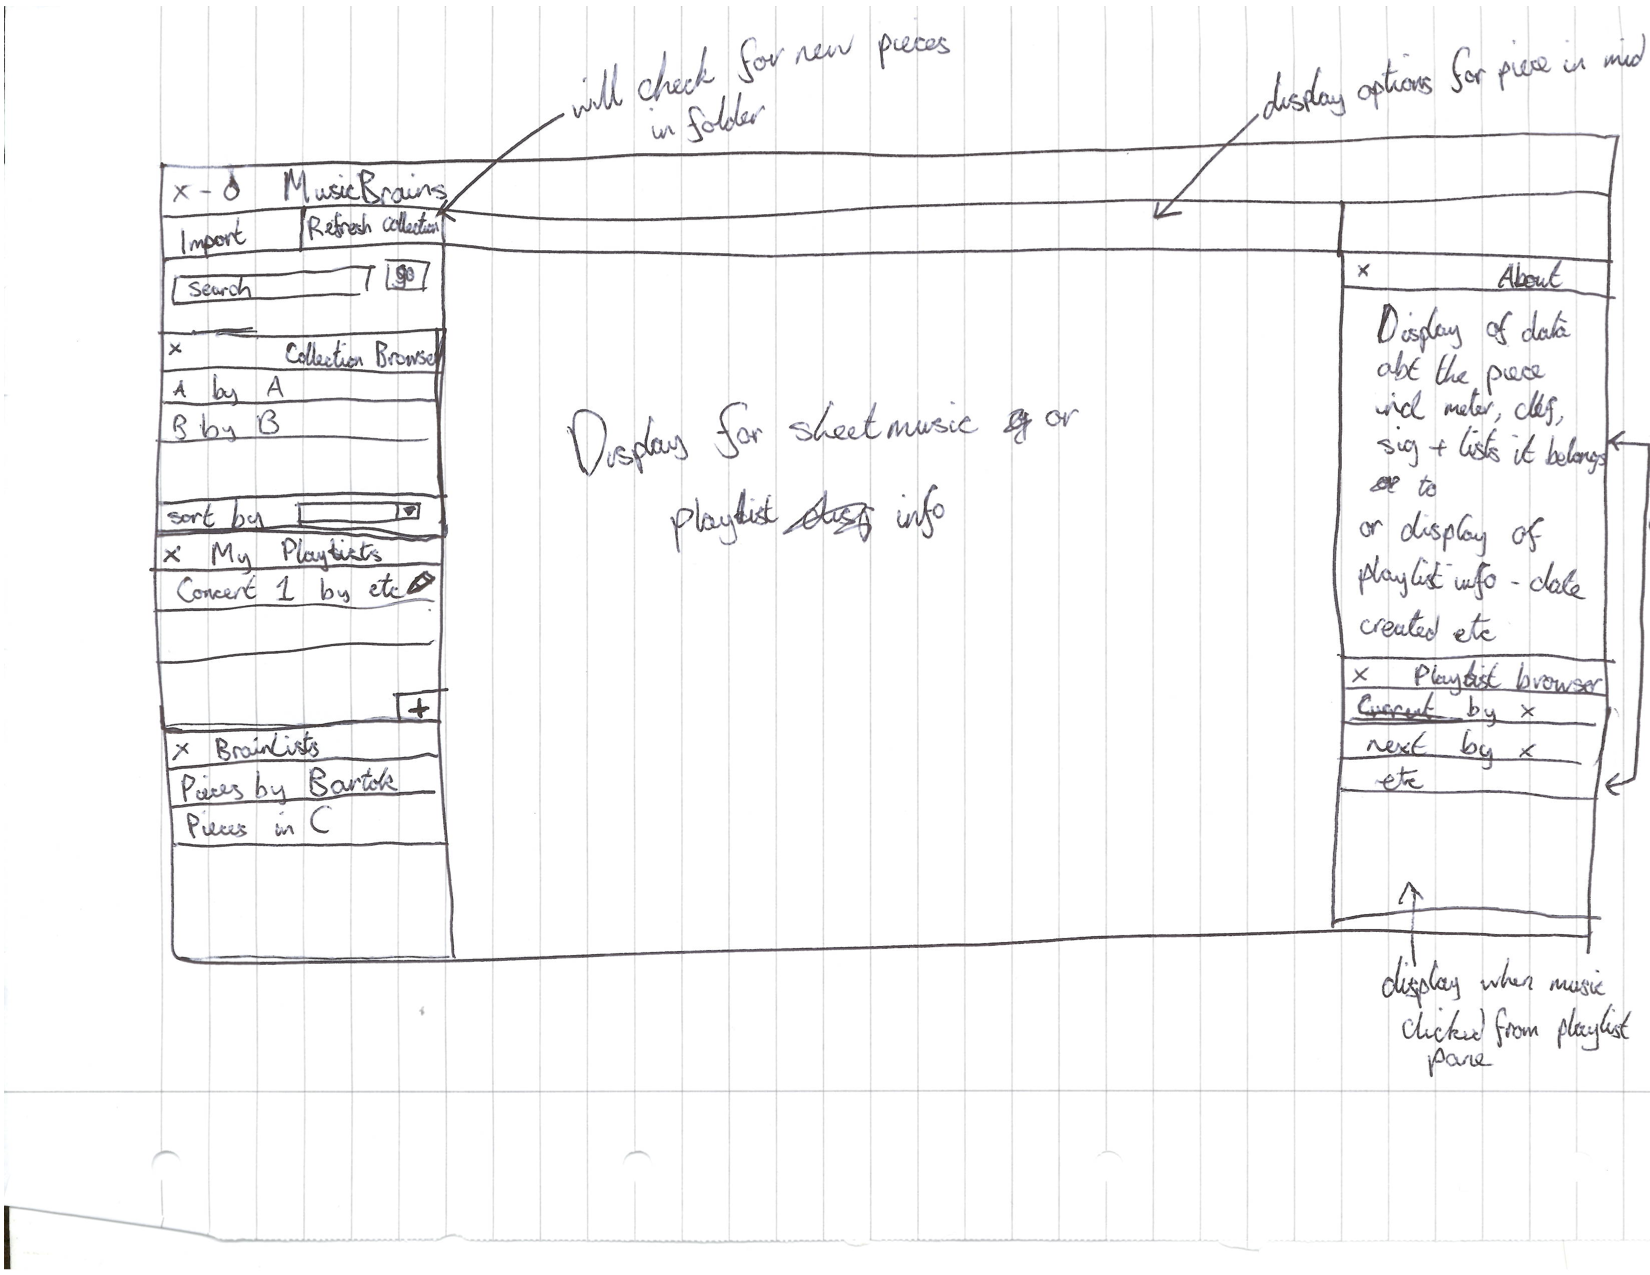
\includegraphics[width=380pt]{main_view.png}
\end{center}

The above image shows the main view of the application. Various panes to the left can be closed using the X button and show different ways the music can be displayed, either as individual units or as playlists. The panes to the right display content based on what is selected for display in the middle, larger window, generally either a playlist or a singular piece of sheet music. Updates to these panes and various pop up boxes associated with different buttons in the display are in the appendices.
\subsubsection{Musician feedback survey}
In order to understand how well this user interface works with a variety of users, a survey was designed which will be given to a selection of musicians, who will feedback on how easy the UI is to use and any updates which should be made to improve it. This feedback session will be performed after the initial sketches are made into a virtual user interface with no back end connected to the buttons. An example survey is provided in the appendices.
\subsection{Test Design}
\section{Project Management Review}
\subsection{Current progress}

During the initial stages of the project, time was dedicated to researching the appropriate language to use, the file format and the methods and algorithms used by other packages. This involved looking at the projects done in the field of music in Python previously, such as Music21 \parencite{Music21}, and other projects listed on the Python Foundation website \parencite{pmus}. 

Many important decisions were made from this research period, such as the decision to use Lilypond to typeset music files rather than create a new algorithm and the research of MusicOCR options available, leading to the decision that MusicOCR is too big a topic for this project to create a new algorithm.


After this research period, class diagrams were drawn and some initial code implementation for the rendering and metadata objectives was developed. It was decided after this initial stage to use Test Driven Development, as the code base and algorithm for loading in a music file was becoming hard to confirm crucial details were being parsed correctly. A set of unit tests were written for the initial implementation, and from this point onward the methodology was applied.

\begin{figure}[h]
    \centering
    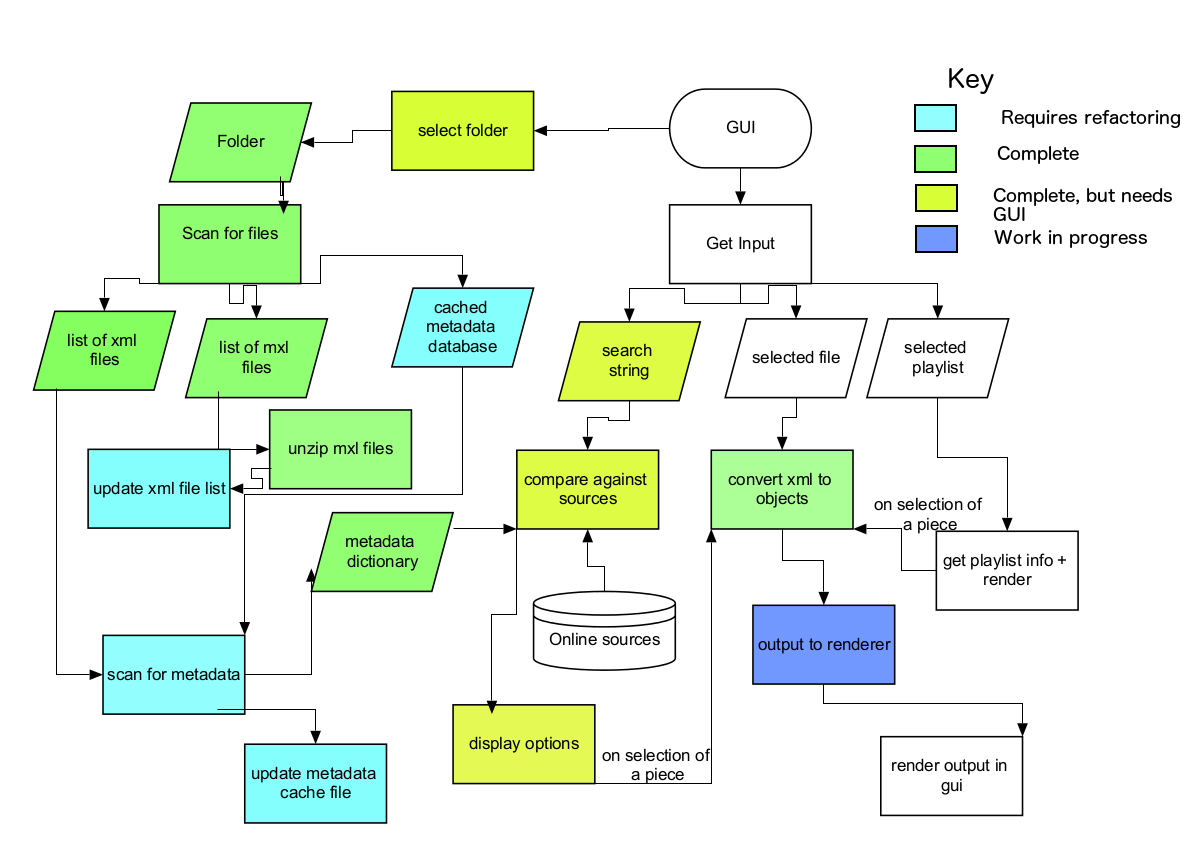
\includegraphics[width=420pt]{flowchart-progress.png}
    \caption{Flowchart colour coded according to progress}
    \label{fig:colours}
\end{figure}
Figure \ref{fig:colours} shows the flowchart shown in figure \ref{fig:flow} colour coded to show progress. 

Of the areas shaded in light blue, to indicate the area needs refactoring, the cached metadata database is currently stored as a serialised python object. In order to make this as extendible and portable as possible, this will need to be refactored to using an SQLite file to be considered completed, as stipulated in section 3.3.3. SQLite is a light implementation of an SQL database stored as a single file, which should be relatively simple to implement in other languages as it is standardised.
\subsection{Adjustments made}
During the initial planning phase the developer included coursework deadlines. However, concessions were not considered at times when other coursework should and did take precedence. In particular, the week before the Languages and Compilers coursework deadline, work was solely focussed on development for this coursework.

Furthermore, the initial research phase was very open ended and some topics took less time than was intended than others. In this case, the developer used the extra time working on other coursework, though in the future adjustments to move future tasks forward should be done instead.

Thirdly, the development methodology in use now is Test Driven Development, meaning that the testing phases between prototype developments can be changed to specified testing sections, such as user interface testing and stress testing, rather than functionality testing.

Finally, the first two weeks of term were affected by jet lag from attending a conference in the United States, which meant that documentation and development suffered a little. Again, the developer was aware that this could occur and should have considered it as a potential risk, though this particular problem will not occur again in the course of the project.

Considering these factors, the revised time plan in figure \ref{fig:timeplan} includes time dedicated solely to coursework for other modules where deadlines arise, and attempts to more clearly define tasks which are open ended.
\begin{landscape}
\subsection{Revised timeplan}
\begin{figure}[H]
	\centering
  \fbox{
   \scalebox{0.3}{\includegraphics*[viewport=0 2538 1892 3808]{timeplan}}
  }
\end{figure}
\begin{figure}[h]
\centering
 \fbox{
   \scalebox{0.3}{\includegraphics*[viewport=0 1269 1892 2538]{timeplan}}
  }
\end{figure}
\begin{figure}[h]
\centering
  \fbox{
   \scalebox{0.3}{\includegraphics*[viewport=0 0 1892 1269]{timeplan}}
  }
 \caption{Updated timeplan}
 \label{fig:timeplan}
\end{figure}
\end{landscape}

\begin{appendices}
\section{Mind map of elements of Music}
\section{Initial class diagram}
\section{Revised computerised class diagram}
\section{Initial User Interface Design}
\section{User Interface Feedback survey}
\section{Revised User Interface Design}
\end{appendices}
\section{References}
\printbibliography[heading=none]

\end{document}
